% Main LaTeX file for the Morpho User Guide 
% 
% Designed to be compiled using pdflatex, as in:
%  $ pdflatex MorphoUserGuide.tex
%
% The section-specific tex files (referenced in the 'include' statements
% below) must be present in the current directory, and all included
% graphics must be present in ./images.
%
% TODO:
% - compress figures to reduce file size?
%
% Jim Regetz
% NCEAS
% 
%
\documentclass[11pt]{article}

% load required packages
\usepackage{graphicx}
\usepackage{array}
\usepackage{color}
\usepackage[hang,small,bf]{caption}
\usepackage{framed}
\usepackage[colorlinks=true,linkcolor=blue,urlcolor=magenta,breaklinks]{hyperref}

% use Helvetica
\renewcommand{\rmdefault}{phv}

% use #.#-style figure numbering
\renewcommand{\thefigure}{\thesection.\arabic{figure}}

% make autoref use 'section' label for all section levels
\def\subsectionautorefname{section}
\def\subsubsectionautorefname{section}

% make URLs have same font as regular text
\urlstyle{same}

% define shadedcolor for shaded frame environment
\definecolor{shadecolor}{gray}{0.95}

\begin{document}

  \pagestyle{empty}

  % title
  \begin{titlepage}
    \begin{center}
    
\includegraphics[width=2cm]{images/logo-morpho.png}\\[0.5cm]
    \textsc{\LARGE Morpho 1.10.1 User Guide}\\[1cm]
    \textsc{Guide Version 1.5}\\
    \textsc{November 2013}
    \vfill
    
\includegraphics[width=1.5cm]{images/logo-nceas.jpg}\\[0.5cm]
    \textsc{National Center for Ecological\\Analysis and Synthesis}\\[1cm]
    
\includegraphics[width=1.5cm]{images/logo-knb.jpg}\\[0.2cm]
    \textsc{Knowledge Network for Biocomplexity}
    \end{center}
  \end{titlepage}
  \pagebreak

  % table of contents
  \tableofcontents
  \pagebreak

  % main content
  \section{Introduction}

The Morpho User Guide is provided to assist scientists who want to use
the Morpho application locally or both locally and on a network to
manage, discover, and share data sets.

If you cannot find the information you are looking for in the User
Guide, please contact \href{mailto:morpho-dev@ecoinformatics.org}
{\nolinkurl{morpho-dev@ecoinformatics.org}}.

\subsection{What is Morpho?}

Created for scientists, Morpho is a user-friendly application designed
to facilitate the creation of metadata (information that describes your
data) so that you and others can easily locate and determine the nature
of a wide range of data sets. By specifying some basic information (a
title and abstract, for example) about your data in a uniform,
standardized way, you or any one you have granted permission to access
your data will be able to find and view the data. When you create a
metadata file that explains what your data represent and how they are
organized, you are not only better able to manage the data, you help
other scientists discover and understand them too. 

Morpho interfaces with the Knowledge Network for Biocomplexity (KNB)
Metacat server, which is essentially a server from which scientists can
upload, download, store, query and view relevant metadata and data. Once
you have annotated your data with metadata, you can choose to upload
your data--or just your data description (the metadata)--to the Metacat
server, where they can be accessed from the web by selected colleagues
or by the public if you so choose. Data stored on the Metacat server is
saved on several geographically separate servers, ensuring that data are
archived securely.

Morpho and Metacat are part of the Knowledge Network for Biocomplexity
(KNB), a national network intended to facilitate ecological and
environmental research on biocomplexity.

\subsection{Terms you need to know}

Throughout this guide, we refer to \hyperref[sec:metadata]{metadata}
and \hyperref[sec:data package]{data package}. Both terms are briefly
defined below.

\subsubsection{Metadata} \label{sec:metadata}

In Morpho, the metadata--or data describing data--contains information
about the content of a data set (its owner, administrator, geographic
extent, units, etc) as well as who has access to the data (the owner,
selected users, or the public). This information is stored in a file
that conforms to the Ecological Metadata Language (EML) specification,
which is commonly used to exchange information among scientists across
the world.

When you use one of Morpho's easy-to-use wizards to create a metadata
file, Morpho automatically takes the values you enter and generates the
metadata file in the proper format. The metadata file is stored on your
local system and/or on the KNB network. Metadata can be "packaged" with
the data set, or can stand alone—much like an abstract describing the
contents of a paper. 

The Morpho wizards create metadata files using a subset of Ecological
Metadata Language (EML), a metadata specification developed by ecology
discipline but that has since gained wider usage. EML is based on prior
work done by the Ecological Society of America and associated efforts
(Michener et al., 1997, Ecological Applications 7: 330-342). For more
information about EML, see
\url{http://knb.ecoinformatics.org/software/eml/}


\subsubsection{Data Package} \label{sec:data package}

Data packages are the logical units that Morpho creates to represent a
collection of metadata and (optionally) data files. At its most basic, a
data package consists only of high-level documentation: metadata about a
data collection's title and abstract, keywords, people and
organizations, usage rights, research project information, coverage
details, methods and sampling, and access information. Once a basic data
package has been created, you can add metadata for the individual data
tables (row and column information) and optionally include the data
tables themselves in the package. 

Data packages can be uploaded to the KNB network and shared with
colleagues, or stored locally on your system.


    \setcounter{figure}{0} 
  \section{Getting Started}

Morpho is available for Linux, Windows, and Mac. 

\subsection{System Requirements}

Recommended system requirements for running Morpho: 
\begin{itemize}
 \item a minimum of 256 MB of RAM 
 \item a minimum of 700MHz CPU 
 \item Java 1.6 or greater 
\end{itemize}

Morpho will run on slower systems with less RAM, but some operations may
be very slow. More RAM is especially useful if there are a large number
of local data packages, since local data are cached in RAM at startup. 

\subsection{Downloading and Installing Morpho}

To download Morpho, go to
%\href{http://knb.ecoinformatics.org/morphoportal.jsp}
%{\nolinkurl{http://knb.ecoinformatics.org/morphoportal.jsp}}
\url{http://knb.ecoinformatics.org/morphoportal.jsp}
and choose the link corresponding to your platform (Morpho can be used
on Windows, Linux, and Mac). You will need to have Java 1.6 or later
installed on your system.

If you have used a previous version of Morpho, we recommend that you
uninstall it before installing a new version. You will be able to
uninstall the old version and install the newer one without losing any
locally stored data packages. 

Note that Morpho will search and display older EML packages (e.g., 2.0
or Beta 6) as EML 2.0. If a package does not use the latest EML format,
Morpho will prompt users to transform the EML to the latest version. If
you choose to upgrade the EML to the latest version, you must save the
data package to preserve the changes, at which time the revision number
of the document will be incremented. If a user chooses to upgrade the
EML and the upgraded EML document is invalid (e.g., a required metadata
field is blank), a correction wizard opens to allow users to fix the
problem. For more information, please see \autoref{sec:upgrading-eml}.

\subsection{Before you Begin} \label{sec:before-you-begin}

Before you can start using Morpho, you must create a user profile, which
is used by the application to manage your data packages. You may choose
to create multiple user profiles to manage different collections of
data, or use one profile for all your Morpho work. 

In order to take advantage of Morpho's useful network functionality, you
must also register for the KNB network.  Because you are prompted to
enter information about your KNB account when you create a user profile,
we recommend that you first register with the KNB Network before
creating a user profile.

\subsubsection{Register for the KNB Network} \label{sec:register}

Registering with the KNB network allows you to take advantage of the
advanced storage, access, and querying capabilities provided by the
Metacat server. If you do not have access to the Internet, or you do not
want to register for the KNB, Morpho will still work, but you will only
be able to store your metadata files locally, and will not be able to
log in to the KNB to create or edit data sets that are stored remotely.

To register for the KNB network, go to
\url{http://knb.ecoinformatics.org/}, select the 'Create new account'
link, and fill out the form (\autoref{fig:register-knb}). Write down
your user name and password as you will need this information when you
create a Morpho user profile.

\begin{figure}
  \centering
    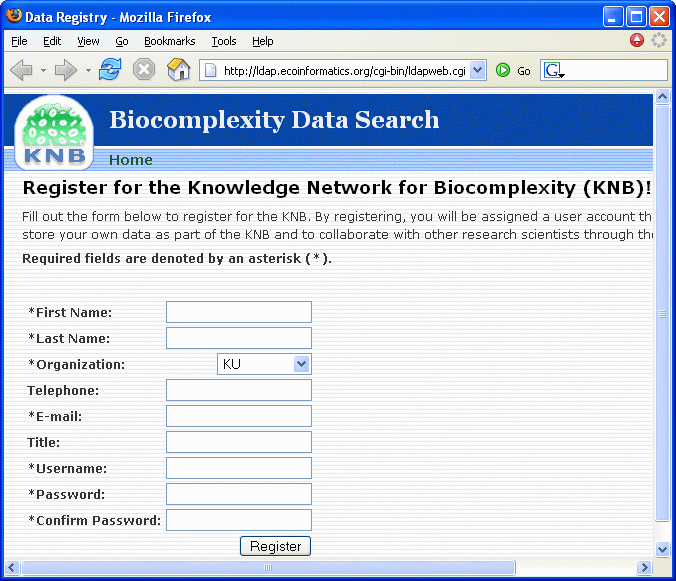
\includegraphics[width=0.7\textwidth]{images/register-knb.png}
  \caption{Registering for the KNB network}
  \label{fig:register-knb}
\end{figure}

\subsubsection{Create a User Profile}

The user profile allows you to use Morpho locally on your personal
computer and, once registered for the KNB (see \ref{sec:register}), to
create, access, edit, and search for metadata and data on the KNB. 

First-time users will automatically be prompted to create a new profile
when they open Morpho. Users upgrading Morpho from a previous version
may also be prompted to create a new profile. To continue using your
old profile(s) (so that your locally-stored data continue to be
visible), simply enter a ``new profile'' with the same user name as the
old one (e.g., if your old profile is named ``jdoe'', then enter
``jdoe'' as the name of the new profile). Click ``Yes'' when prompted,
to confirm that you would like to use the existing profile. Note: You
must be logged in to your computer with the same account under which
your old profile existed.

\paragraph{To create a user profile:}
\begin{enumerate}
  \item On the ``Basic Information'' screen of the New Profile wizard
    (\autoref{fig:new-profile-name}), enter your profile name and your
    first and last names. Your profile name does \emph{not} have to be
    the same as your KNB username. Click ``Next.''

  \begin{figure}
    \centering
      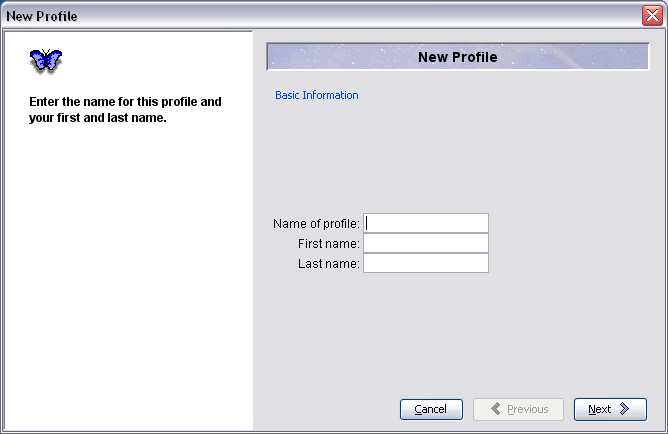
\includegraphics[width=0.7\textwidth]{images/new-profile-name.png}
    \caption{Step 1: Create a profile name.}
    \label{fig:new-profile-name}
  \end{figure}

  \item On the ``Network Account Information'' screen
    (\autoref{fig:new-profile-account}), enter your KNB username and the
    organization you selected when you
    \hyperref[sec:register]{registered for the KNB}. If your
    organization is not listed, click the Refresh button to look up the
    most recent account information. Click ``Next.'' 

  \begin{figure}
    \centering
      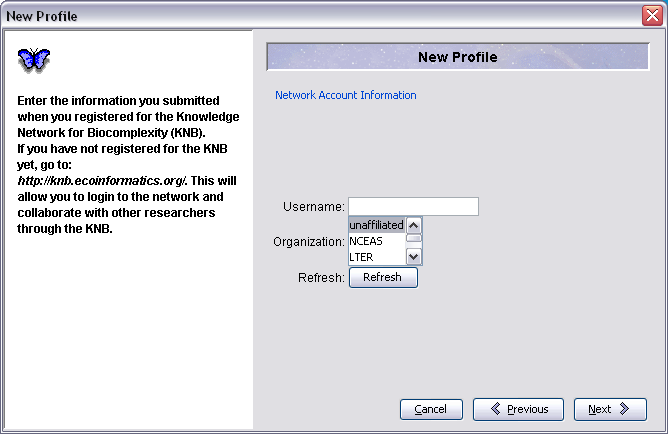
\includegraphics[width=0.7\textwidth]{images/new-profile-account.png}
    \caption{Step 2: Enter your KNB username and organization.}
    \label{fig:new-profile-account}
  \end{figure}

  \item On the ``Data Package Identification'' screen
    (\autoref{fig:new-profile-prefix}), enter a short identifier prefix.
    The identifier prefix will be used to create IDs for metadata
    documents you create in Morpho, and for data tables or other data
    files you import using Morpho. For example, specifying the prefix
    ``jane\_doe'' will result in document IDs like jane\_doe.1.1,
    jane\_doe.2.1, etc. \emph{\textbf{Do not use the reserved prefix
    ``temporary''.}} Other non-alphanumeric characters like periods, 
    commas, and quotation marks are also not allowed in the prefix.

  \begin{figure}
    \centering
      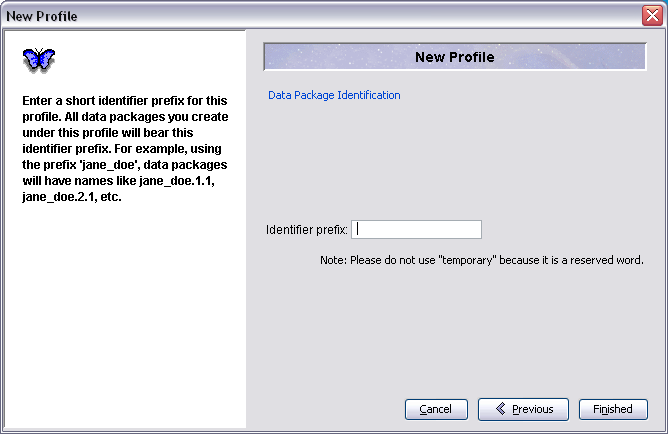
\includegraphics[width=0.7\textwidth]{images/new-profile-prefix.png}
    \caption{Step 3: Specify an identifier prefix.}
    \label{fig:new-profile-prefix}
  \end{figure}

  \item Click ``Finished'' to complete the profile.
\end{enumerate}

\begin{shaded}
  \textbf{NOTE} The Morpho interface currently supports deleting
  profiles that you no longer need through the Remove Profile menu item
  from the File menu (see \autoref{sec:removing-a-profile}).
   \textbf{However, if you delete a profile, you also
  delete all local copies of data packages created or saved using that
  profile}. Unless you first extract the data packages and save them
  elsewhere on your computer (or to a network server, like Metacat), you
  may lose data.
\end{shaded}

\subsection{Logging In}

After you have created a user profile (see
\autoref{sec:before-you-begin}), you will see the Main Morpho screen.
Enter your KNB password in the ``Network Status'' panel and click
``Login'' (\autoref{fig:panel-login}). If you choose not to log in, you
will be able to create, edit, search, access, and manage data that are
stored locally, and may search for public data sets on the KNB network.
However, you will not be allowed to create or edit data sets on the KNB
network.

\begin{figure}
  \centering
    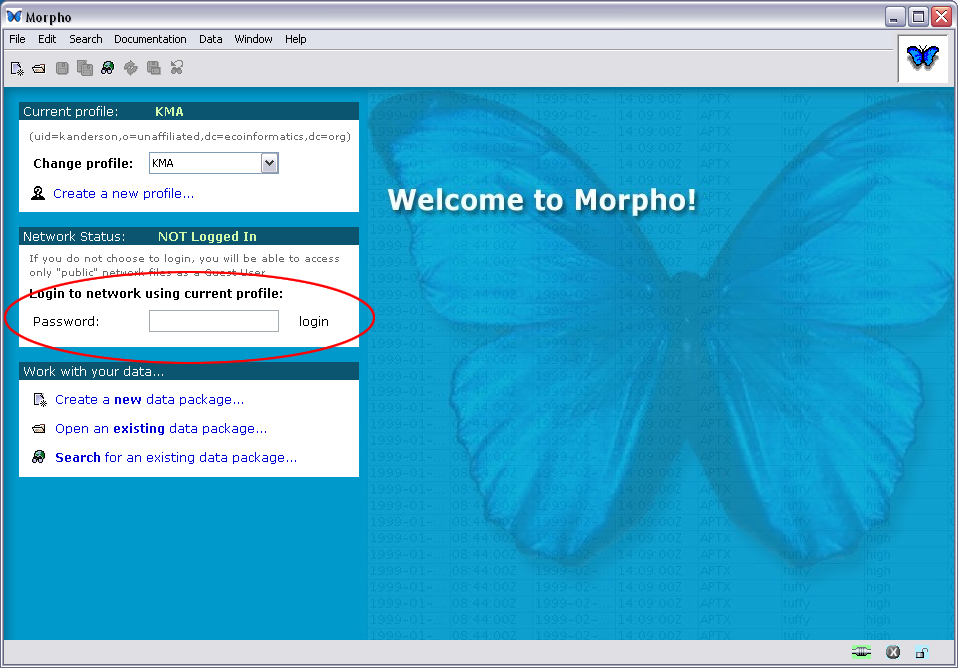
\includegraphics[width=0.7\textwidth]{images/panel-login.jpg}
  \caption{Log in to the KNB network.}
  \label{fig:panel-login}
\end{figure}

\subsection{Removing a profile} \label{sec:removing-a-profile}

Profiles may be removed from Morpho if they are no longer needed.
When you remove a profile, all the metadata and data that has been created 
with that profile is deleted locally. Network copies remain untouched.

\paragraph{To remove a user profile:}
\begin{enumerate}
  \item From the File menu, choose ``Remove profile''
  \item Select the profile that should be removed (\autoref{fig:remove-profile-select}).
  Note: The current active profile cannot be removed (switch to a different profile in order to remove it).
  
  
  \begin{figure}
  \centering
    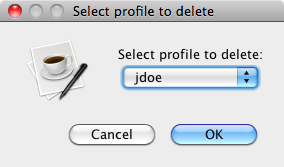
\includegraphics[width=0.7\textwidth]{images/remove-profile-select.png}
  \caption{Select profile to remove}
  \label{fig:remove-profile-select}
\end{figure}
  
  \item Confirm the removal in the dialog box (\autoref{fig:remove-profile-confirm}).
  \begin{figure}
  \centering
    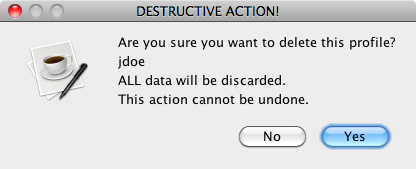
\includegraphics[width=0.7\textwidth]{images/remove-profile-confirm.png}
  \caption{Confirm profile removal.}
  \label{fig:remove-profile-confirm}
\end{figure}

\end{enumerate}


    \setcounter{figure}{0} 
  \section{The Morpho Interface: The Main Screen} \label{sec:main}

After you have opened Morpho and created a profile, you will see the
Main Morpho screen (\autoref{fig:main}). The screen provides access to
all of the most commonly used Morpho functionality, via the three panels
on the left side of the screen (\nameref{sec:panel-profile},
\nameref{sec:panel-network-status}, and \nameref{sec:panel-work}), the
menu items in the \nameref{sec:menu-bar}, and the shortcut buttons in
the \nameref{sec:toolbar}. The \nameref{sec:status-bar} at the bottom of
the screen contains information about the current status of various
Morpho settings and parameters.

\begin{figure}
  \centering
    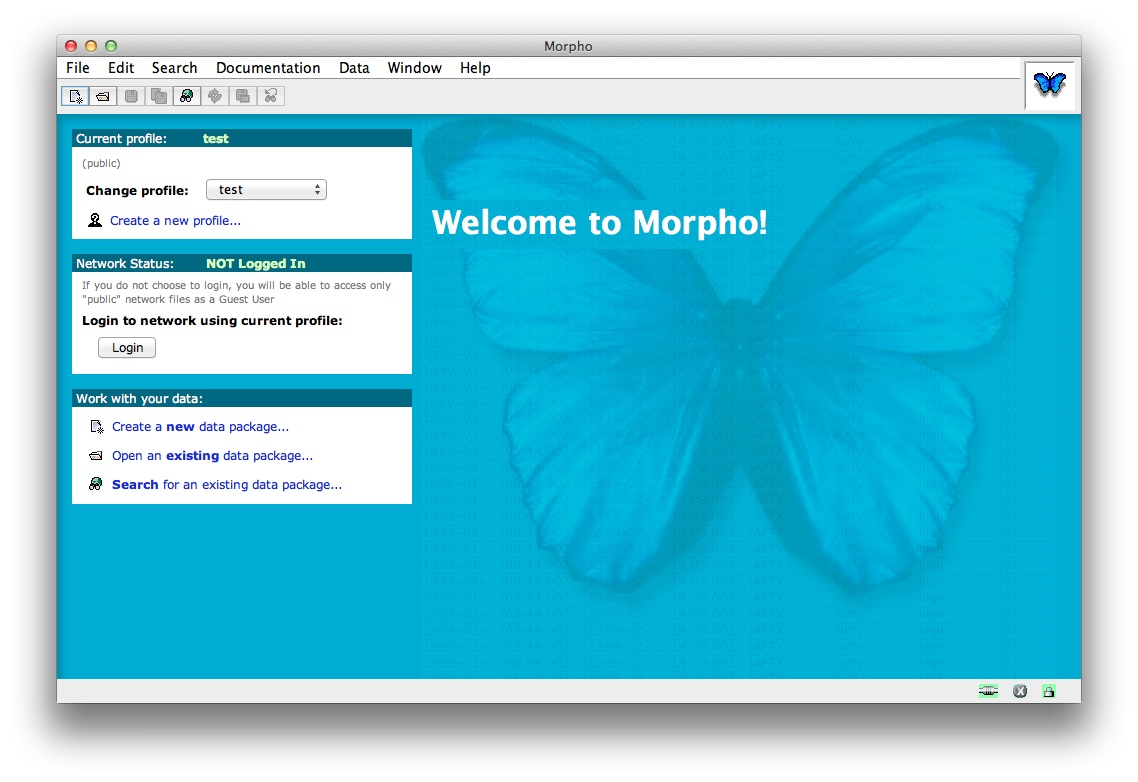
\includegraphics[width=0.7\textwidth]{images/main.jpg}
  \caption{Main Morpho screen with interface components highlighted.}
  \label{fig:main}
\end{figure}

\subsection{Panels}

The Main Morpho screen contains three panels designed to help you easily
log in to a network, select or change a profile, and access the most
common Morpho functions.

\subsubsection[Current profile]{Current Profile Panel}
\label{sec:panel-profile}

The Current Profile panel (\autoref{fig:panel-profile}) contains
information about your current user profile as well as the KNB login
information associated with that profile. Your KNB username is the name
appearing after the ``uid='' just below the title bar of the ``Current
Profile'' panel. 

\begin{figure}
  \centering
    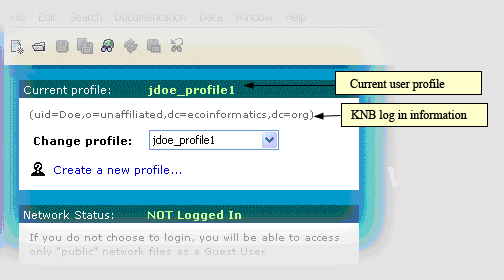
\includegraphics[width=0.7\textwidth]{images/panel-profile.jpg}
  \caption{The Current Profile panel from the Main Morpho screen.}
  \label{fig:panel-profile}
\end{figure}

Use the drop-down menu beside ``Change profile\ldots'' to select a
different profile, or click the ``Create a new profile\ldots'' link to
create a new profile. You may wish to create new profiles to allow
different users to use the same copy of Morpho or to manage different
projects, for example.
%TODO: say something *here* about removing profiles? (we briefly say
%something in the 'getting started' section already, although it seems
%less relevant there because the section is otherwise only about the
%stuff you do when you start Morpho for the first time

\subsubsection[Network Status]{Network Status Panel}
\label{sec:panel-network-status}

The Network Status panel displays the current network status and allows
you to log in and out of the KNB network. The panel offers different
options depending on whether or not you are logged in to the network
(\autoref{fig:panel-network-status}).

\begin{figure}
  \centering
    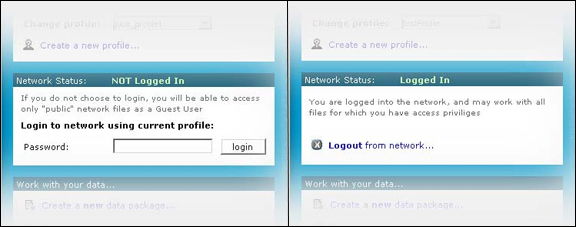
\includegraphics[width=0.7\textwidth]{images/panel-network-status.jpg}
  \caption{The Network Status panel from the Main Morpho screen. The
    image on the left displays the panel as it appears when not logged
    in to the KNB network. The image on the right displays the panel as
    it appears when logged in to the network.}
  \label{fig:panel-network-status}
\end{figure}

If you are not logged in to the KNB network, you can log in by typing
your KNB password in the ``Password'' field and clicking the ``Login''
button. You will be logged in with the KNB username associated with the
current profile (the KNB account information is displayed in the
``Current Profile'' panel). Note that the KNB username is not necessarily
the same as your user profile name. Log out at any time by clicking 
``Logout from network.''

\subsubsection[Work with your data\ldots]{Work with Your Data Panel}
\label{sec:panel-work}

The ``Work with your data\ldots'' panel (\autoref{fig:panel-work})
allows you to easily access the most common features of Morpho. Click
any of the links \hyperref[sec:creating]{Create a new data package},
\hyperref[sec:viewing]{Open an existing data package}, or
\hyperref[sec:searching]{Search for an existing data package} (both
locally and on the KNB network) to start working. Detailed descriptions
of these functions are provided later in the guide.

\begin{figure}
  \centering
    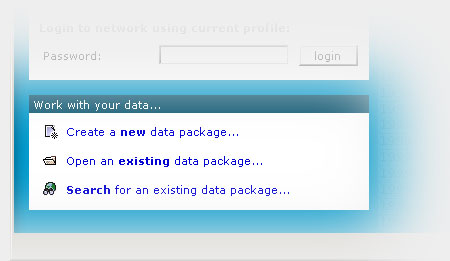
\includegraphics[width=0.7\textwidth]{images/panel-work.jpg}
  \caption{The Work with your data panel from the Main Morpho screen.}
  \label{fig:panel-work}
\end{figure}


\subsection{Menu bar} \label{sec:menu-bar}

The menus in the Menu bar allow you to access all the available Morpho
operations. Each of the menus -- File, Edit, Search, Documentation,
Data, Window, and Help -- is discussed in more detail below.

\subsubsection{File menu} \label{sec:menu-file}

Use the File menu (\autoref{fig:menu-file}) to create a new data
package, open an existing data package, log in and out of the KNB
network, create a new user profile, save a data package, delete a data
package, print documentation, set preferences, and exit Morpho, among
other options. 

\begin{figure}
  \centering
    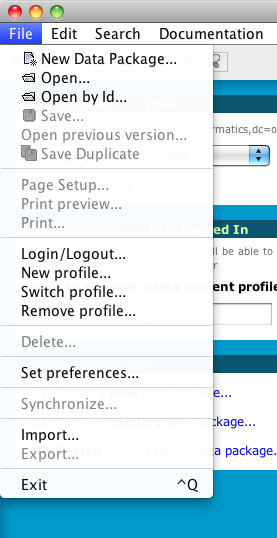
\includegraphics[width=0.5\textwidth]{images/menu-file.png}
  \caption{The File menu}
  \label{fig:menu-file}
\end{figure}

\subsubsection{Edit menu} \label{sec:menu-edit}

Use the Edit menu (\autoref{fig:menu-edit}) to cut, copy or paste items,
as well as reverse changes you have made to a data table or to a set of
data tables.

\begin{figure}
  \centering
    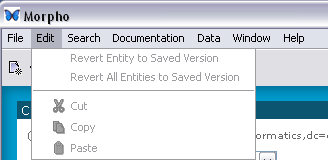
\includegraphics[width=0.5\textwidth]{images/menu-edit.jpg}
  \caption{The Edit menu}
  \label{fig:menu-edit}
\end{figure}

\subsubsection{Search menu} \label{sec:menu-search}

Use the Search menu (\autoref{fig:menu-search}) to search for data
packages, save a search for future use, refine a search by changing
search parameters, or refresh the current search. 

\begin{figure}
  \centering
    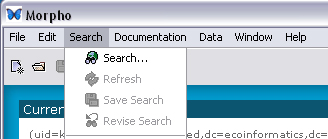
\includegraphics[width=0.5\textwidth]{images/menu-search.jpg}
  \caption{The Search menu.}
  \label{fig:menu-search}
\end{figure}

\subsubsection{Documentation menu} \label{sec:menu-documentation}

Use the Documentation menu (\autoref{fig:menu-documentation}) to add,
delete, or change a variety of different types of documentation
(metadata) for your data package. 

\begin{figure}
  \centering
    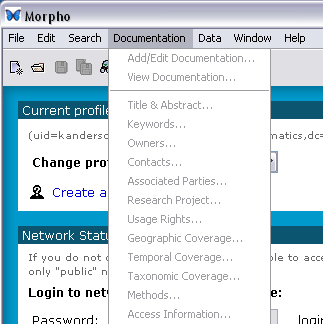
\includegraphics[width=0.5\textwidth]{images/menu-documentation.jpg}
  \caption{The Documentation menu}
  \label{fig:menu-documentation}
\end{figure}

\subsubsection{Data menu} \label{sec:menu-data}

Use the Data menu (\autoref{fig:menu-data}) to import data (e.g., a data
table or an image) or create a data table. You can also edit and
manipulate the data in a data table or add or edit the table
documentation. 

\begin{figure}
  \centering
    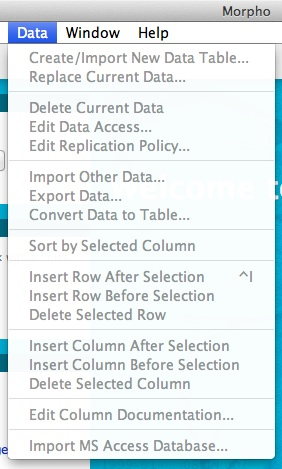
\includegraphics[width=0.5\textwidth]{images/menu-data.jpg}
  \caption{The Data menu}
  \label{fig:menu-data}
\end{figure}

\subsubsection{Window menu} \label{sec:menu-window}

Use the Window menu (\autoref{fig:menu-window}) to view open Morpho
windows. 

\begin{figure}
  \centering
    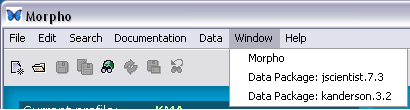
\includegraphics[width=0.5\textwidth]{images/menu-window.jpg}
  \caption{The Window menu.}
  \label{fig:menu-window}
\end{figure}

\subsubsection{Help menu} \label{sec:menu-help}

Use the Help menu (\autoref{fig:menu-help}) to access the Morpho User
Guide (which is what you are now reading). The ``About...'' item
contains general information about Morpho. The ``Intro to Metadata...''
document explains what metadata is and why it is important, as well as
some of the challenges associated with creating it, what Ecological
Metadata Language (EML) is, and how it is used. The EML Specification
contains information about each EML module and how it is used.

\begin{figure}
  \centering
    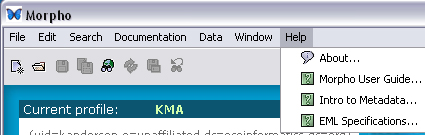
\includegraphics[width=0.5\textwidth]{images/menu-help.jpg}
  \caption{The Help menu}
  \label{fig:menu-help}
\end{figure}
 

\subsection{Toolbar} \label{sec:toolbar}

The Toolbar (\autoref{fig:button-bar-main}) contains shortcut buttons to the
most commonly-used Menu items. Each button is described in
\autoref{tab:button-bar}. To display the purpose of a Morpho button,
simply place your mouse cursor over the button. A small pop-up reminder
will display the purpose of the button.

\begin{figure}
  \centering
    
\includegraphics[width=0.7\textwidth]{images/button-bar-main.png}
  \caption{The Morpho Toolbar}
  \label{fig:button-bar-main}
\end{figure}
 
\begin{table}[ht]
  \centering
  \begin{tabular}{|c|m{0.7\textwidth}|}
  \hline
  \textbf{Button} & \textbf{Description} \\
  \hline
  
\includegraphics[scale=0.7]{images/button-new-dp.png} &
  The ``Create a new data package'' button starts a wizard that guides
  you through the process of creating a new data package. \\
  \hline
  
\includegraphics[scale=0.7]{images/button-open.png} &
  The ``Open\ldots'' button opens an existing data package (provided you
  have adequate access permissions). \\
  \hline
  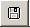
\includegraphics[scale=0.7]{images/button-save.png} &
  The ``Save\ldots'' button saves the current data package either
  locally or on the network. \\
  \hline
  
\includegraphics[scale=0.7]{images/button-duplicate.png} &
  The ``Duplicate this data package and save locally'' button copies the
  current data package. The duplicate can be used as a template to
  create similar data packages. \\
  \hline
  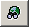
\includegraphics[scale=0.7]{images/button-search.png} &
  The ``Search for data'' button begins the data package search process.
  If logged in to the KNB, you can search both locally and on the KNB
  network. \\
  \hline
  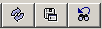
\includegraphics[scale=0.7]{images/button-bar-search.png} &
  The ``Refresh…'', ``Save search,'' and ``Revise search'' buttons are
  enabled only when the screen contains search results. \\
  \hline
  \end{tabular}
  \caption{The Toolbar buttons}
  \label{tab:button-bar}
\end{table}


\subsection{Status Bar} \label{sec:status-bar}

The status bar at the bottom of the Morpho window
(\autoref{fig:status-bar}) contains information about the current status
of various Morpho settings and parameters.

\begin{figure}
  \centering
    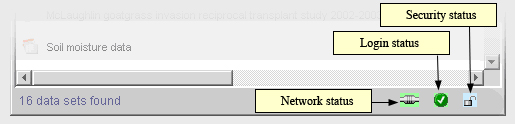
\includegraphics[width=0.7\textwidth]{images/status-bar.jpg}
  \caption{The Morpho Status bar.}
  \label{fig:status-bar}
\end{figure}

\subsubsection*{Network Status}
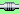
\includegraphics[scale=0.9]{images/indicator-online.png} \hspace{1em}
  Network connection available\\

\includegraphics[scale=0.9]{images/indicator-offline.png} \hspace{1em}
  Network connection not available

\subsubsection*{Login Status}

\includegraphics[scale=0.9]{images/indicator-logged-in.png} \hspace{1em}
  Logged in to network\\

\includegraphics[scale=0.9]{images/indicator-not-logged-in.png} \hspace{1em}
  Not logged in to network

\subsubsection*{Security}

\includegraphics[scale=0.9]{images/indicator-ssl.png} \hspace{1em}
  Using secure (SSL) connection\\

\includegraphics[scale=0.9]{images/indicator-nossl.png} \hspace{1em}
  Not using secure (SSL) connection


    \setcounter{figure}{0} 
  \section{Opening and Viewing a Data Package} \label{sec:viewing}

Existing data packages, which consist of metadata and (optionally) the
data set described by the metadata, are easily opened and viewed in
Morpho. Whether your data package is stored locally, on the network, or
both, you can easily open it with Morpho's Data Package viewer. If you
have permission to access the data, you can also open data packages
created by other scientists. 

\subsection{Opening Data Packages}

To open a data package that you have created, use one of the following
techniques:

\begin{itemize}
  \setlength{\parskip}{1pt}
  \item click the ``Open an existing data package...'' on the ``Work
    with your data'' panel on the Main Morpho screen,
  \item select the ``Open'' menu item from the File menu,
  \item click the 
\includegraphics[scale=0.7]{images/button-open.png}
  icon in the Toolbar.
\end{itemize}

You will then see a listing of the available data packages
(\autoref{fig:open-dp}). Available data packages include those which you
previously created using the current profile and/or under the current
KNB username, along with a fictitious sample data package included with
Morpho -- ``Population sampling data for zooplankton in the Great Lakes,
2000''.

\begin{figure}
  \centering
    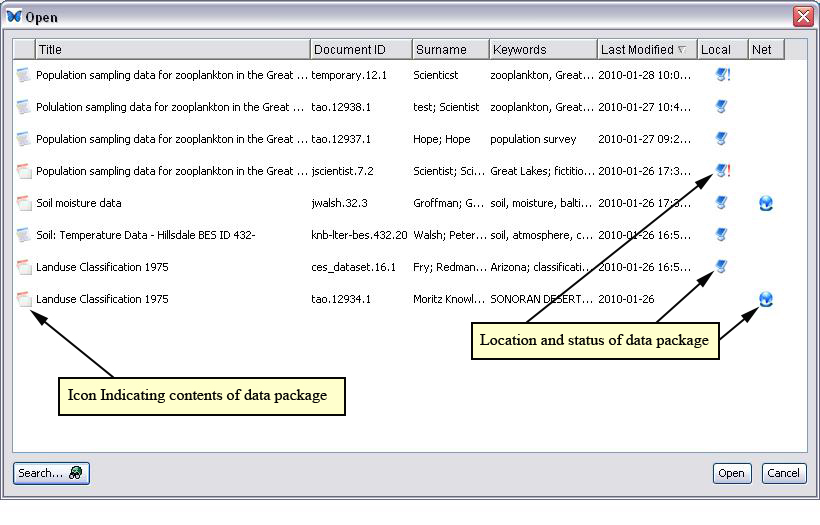
\includegraphics[width=0.7\textwidth]{images/open-dp.jpg}
  \caption{An example listing of available data packages displayed in
    Morpho's Open screen.}
  \label{fig:open-dp}
\end{figure}

The icons in the first column of the Open Data Package screen tell you
if the package contains:
\begin{itemize}
  \parskip 3pt
  \itemsep 0pt
  \item[] 
\includegraphics[scale=0.7]{images/indicator-hasdata.png}
    Data and documentation
  \item[] 
\includegraphics[scale=0.7]{images/indicator-hasnodata.png}
	Documentation only 
\end{itemize}

Icons in the last two columns indicate the location and status of the
package:
\begin{itemize}
  \parskip 3pt
  \itemsep 0pt
  \item[] 
\includegraphics[scale=0.7]{images/indicator-dp-local.png}
  Local data package
  \item[] 
\includegraphics[scale=0.7]{images/indicator-dp-incomplete.png}
  Saved incomplete data package
  \item[] 
\includegraphics[scale=0.7]{images/indicator-dp-network.png}
  Network data package
  \item[] 
\includegraphics[scale=0.7]{images/indicator-dp-recovered.png}
  Recovered incomplete data package
\end{itemize}

For more information about saved and recovered incomplete data package,
please see \autoref{sec:dp-saveforlater} and
\autoref{sec:dp-recover}.

Select a data package to open (or open the fictitious sample package
``Population sampling data for zooplankton in the Great Lakes, 2000'').
To open a selected package, click the ``Open'' button located at the
bottom right of the screen, or double-click the selected data package,
or right-click the data package and select ``Open Package''
(\autoref{fig:menu-dp-rightclick}). You can also open an earlier version
of the data package (if any exist) by right-clicking the package and
selecting ``Open Previous Version.'' Note that one or more previous
versions of the data package may be unavailable, for example, a version
saved only locally on a different computer. The Refresh command updates
the listing of available packages.

\begin{figure}
  \centering
    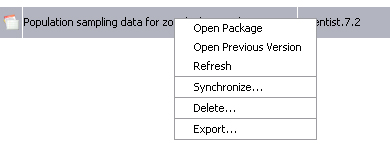
\includegraphics[width=0.7\textwidth]{images/menu-dp-rightclick.jpg}
  \caption{Right-click a data package to open an action menu.}
  \label{fig:menu-dp-rightclick}
\end{figure}

\begin{shaded}
  \textbf{NOTE} Morpho automatically displays data packages stored in
  earlier versions of EML (e.g., 2.0 or Beta 6) as EML 2.0. If a package
  does not use the latest EML format, Morpho will prompt users to
  transform the EML to the latest version. If you choose to transform
  the EML, you will need to save the data package to preserve the
  changes, at which time the revision number of the document will be
  incremented. If the updated EML document is invalid (e.g., a required
  metadata field is blank), a correction wizard opens to allow users to
  fix the problem. For more information, please see
  \autoref{sec:upgrading-eml}.
\end{shaded}

\subsubsection*{Opening a Shared Data Package}

To locate and view data packages other than those you have created, use
the \hyperref[sec:searching]{Search} feature, which is described later
in this guide. You can only open and view data packages for which you
have been granted permission. If you do not have permission to open a
data package, it will not appear in your search results. 

\paragraph{NOTE}
If you are not logged in to the KNB, but have network access, the only
network data packages that will appear in your search are those that
have ``public'' access privileges. To view additional data sets from the
KNB network, log in to the network.

\subsection{Viewing a Data Package: The Data Package Interface}

When you open a data package, Morpho displays it in the Data Package
interface (\autoref{fig:viewer-table-main}). The Data Package interface
contains the standard Menu bar and Toolbar as well as three panels: the
\nameref{sec:panel-dp-doc}, the \nameref{sec:panel-table}, and the
\nameref{sec:panel-table-doc}.

\begin{figure}
  \centering
    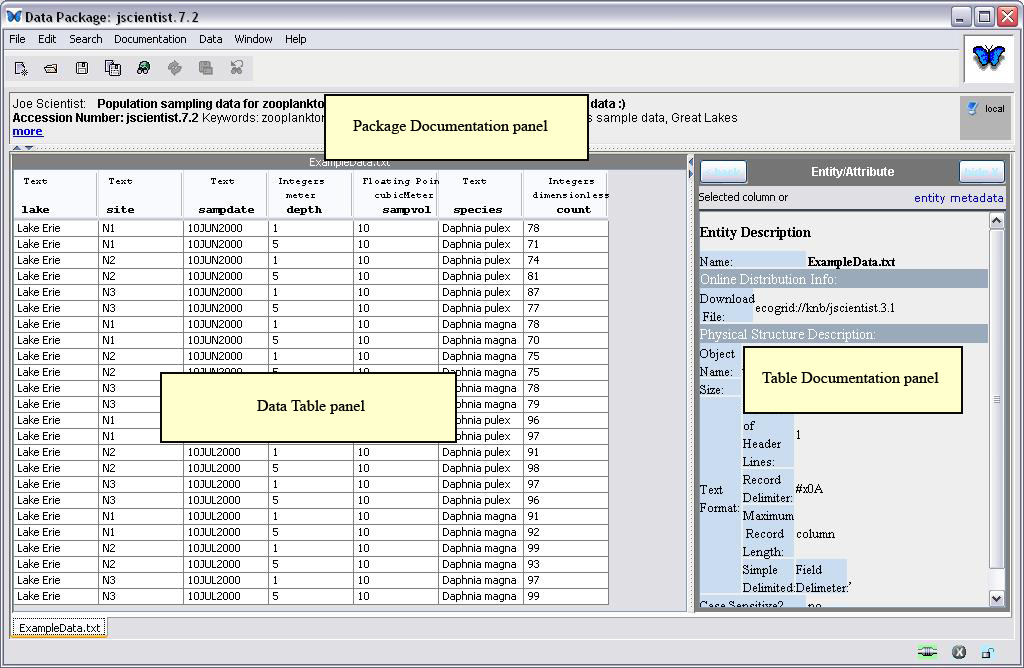
\includegraphics[width=0.7\textwidth]{images/viewer-table-main.jpg}
  \caption{Viewing a data package in Morpho's Data Package interface.}
  \label{fig:viewer-table-main}
\end{figure}

\subsubsection{Package Documentation panel} \label{sec:panel-dp-doc}

The Package Documentation panel contains a brief ``citation-style''
summary of the data package: its title, description, usage information,
etc. The icons on the right side of the panel indicate whether the
package is located on the local machine, on the network, or both
(\autoref{fig:viewer-table-top}). No icons will appear if the data
package has not yet been saved, or has been modified since it was last
saved.
 
\begin{figure}
  \centering
    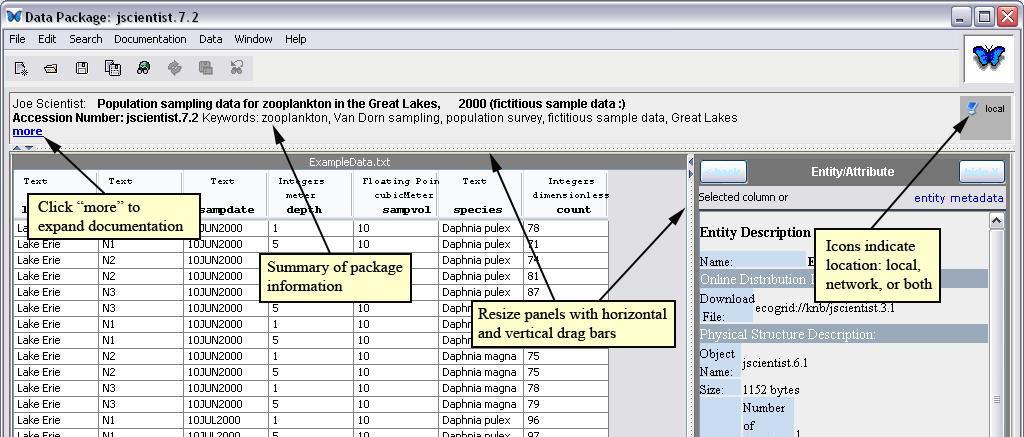
\includegraphics[width=0.7\textwidth]{images/viewer-table-top.jpg}
  \caption{The Data Package panel.}
  \label{fig:viewer-table-top}
\end{figure}

The Package Documentation panel can be expanded to reveal additional
documentation, either by dragging the horizontal drag bar, or by
clicking the ``more'' link (\autoref{fig:viewer-metadata-options}).

\begin{figure}
  \centering
    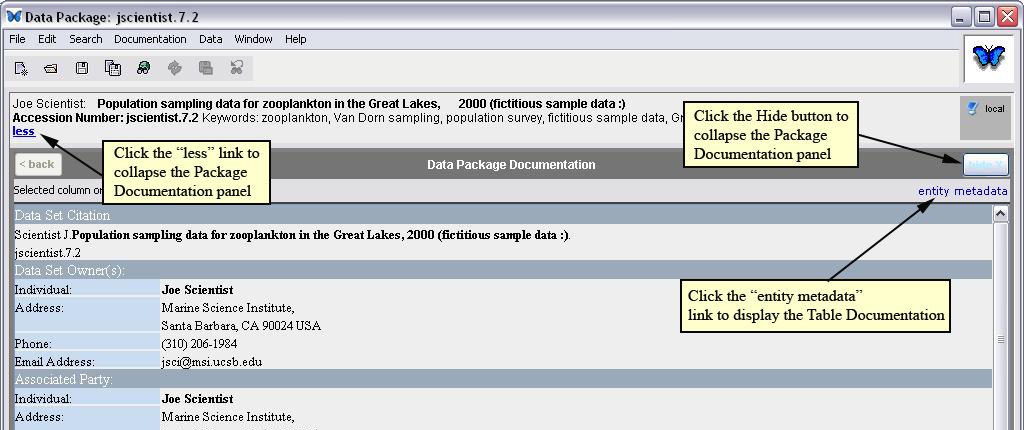
\includegraphics[width=0.7\textwidth]{images/viewer-metadata-options.jpg}
  \caption{The Package Documentation panel after it has been expanded.}
  \label{fig:viewer-metadata-options}
\end{figure}


To collapse the Package Documentation panel:
\begin{itemize}
  \setlength{\parskip}{1pt}
  \item click the ``less'' link 
  \item click the ``hide'' button 
  \item use the mouse to drag the divider bar from the bottom of the
    screen
  \item click the small arrow icon located on the left side of the
    divider bar 
\end{itemize}

\subsubsection{Data Table panel} \label{sec:panel-table}

The Data Table panel (\autoref{fig:viewer-table-bottom}) displays
tabular data in spreadsheet form or image data (for several formats of
image entities). Use the tabs along the bottom of the Data Table panel
to select and view different data tables or image entities contained in
the data package. Use the drag bar on the right side of the panel to
collapse, expand, or change the size of the panel.

\begin{figure}
  \centering
    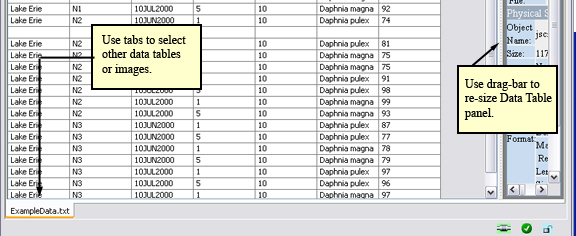
\includegraphics[width=0.7\textwidth]{images/viewer-table-bottom.jpg}
  \caption{The Data Table panel.}
  \label{fig:viewer-table-bottom}
\end{figure}

Click a table cell to edit the data directly. To save changes, use the
Save option under the File menu. To cancel all changes that have been
made to the current panel, choose ``Revert Entity to Saved Version'' under
the Edit menu. Note that it is not currently possible to undo individual
changes made to a panel. To cancel changes that have been made to ALL
data panels, select ``Revert all Entities to Saved Version'' under the
Edit menu.

Right-click the data table to display a menu that allows you to:
\begin{itemize}
  \setlength{\parskip}{1pt}
  \item sort columns 
  \item insert and delete rows 
  \item insert and delete columns 
  \item delete the entire table
  \item add new tables 
  \item add/edit documentation 
\end{itemize}

These same options are also available under the Data menu in the Menu
bar. Read more about using these tools in \autoref{sec:working-with-data}.

\subsubsection{Table Documentation panel} \label{sec:panel-table-doc}

The Table Documentation panel (\autoref{fig:viewer-table-metadata}) displays
documentation for the currently displayed table. Note that tables are
also referred to as ``entities'' in Morpho, using terminology consistent
with database management systems. Similarly, ``attributes'' refers to
table columns (also called ``variables'').

\begin{figure}
  \centering
    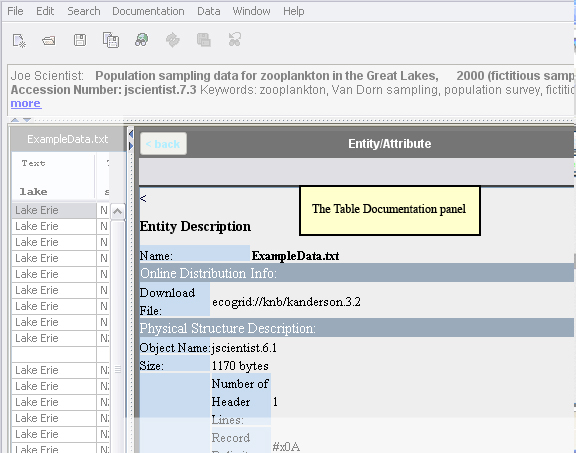
\includegraphics[width=0.7\textwidth]{images/viewer-table-metadata.jpg}
  \caption{The Table Documentation panel (expanded).}
  \label{fig:viewer-table-metadata}
\end{figure}

Click any column header in the Data Table panel to display more specific
information about the selected column in the Table Documentation panel
(\autoref{fig:viewer-column-metadata}).

Return to the table documentation by clicking the Data Table tab at the
bottom of the Data Table panel or on the ``entity metadata'' link. The
``Back'' button works like the back button in a web browser; if you have
viewed several columns of data documentation, the back button will step
back through those column descriptions before returning to the table
documentation. 

To resize the panel, drag the divider bars. Hide or fully expand the
panel by clicking the arrows on the divider bars, or by clicking the
``Hide'' button at the top-right corner. 

\begin{figure}
  \centering
    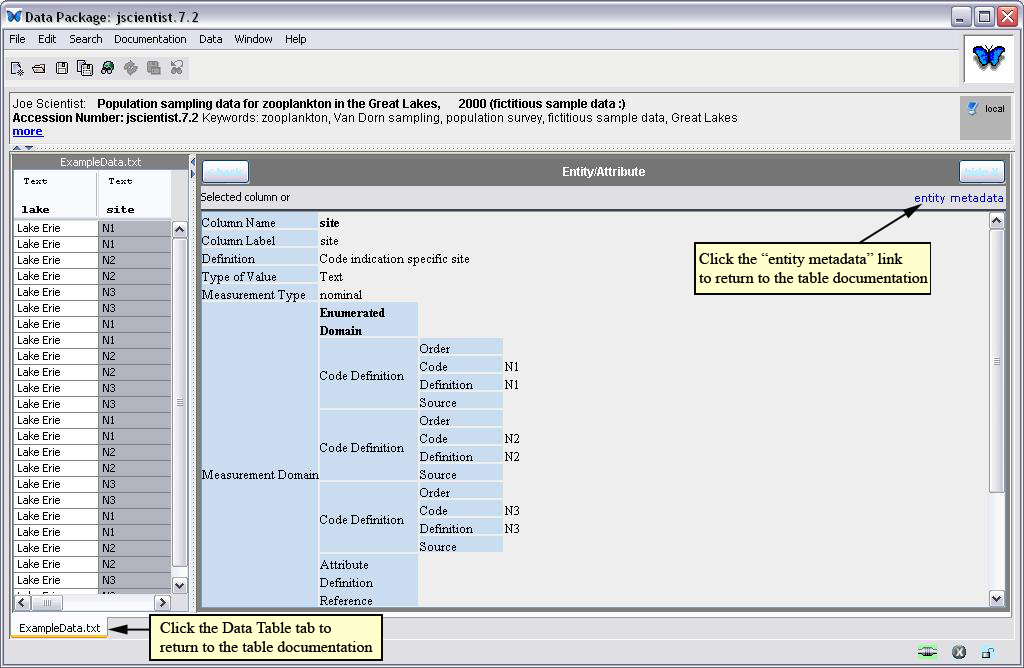
\includegraphics[width=0.7\textwidth]{images/viewer-column-metadata.jpg}
  \caption{Displaying information about a table column in the Table
    Documentation panel.}
  \label{fig:viewer-column-metadata}
\end{figure}


    \setcounter{figure}{0} 
  \section{Searching for Data Packages} \label{sec:searching}

Use Morpho queries to easily locate data packages (your packages and/or
packages shared by other scientists) based on a variety of specified
criteria. Packages can be searched by subject, taxonomic rank, and/or
spatial extent. Combine these major search criteria to further refine
result sets. 

\begin{shaded}
  \textbf{NOTE} 
  If you are not logged in to DataONE but have network
  access, the only network data packages that will appear in your search
  results are those that have "public" access privileges. To view
  additional data sets from the network, log in 
  from the \hyperref[sec:main]{main Morpho screen}.
\end{shaded}

\subsection{Opening the Search Interface and Performing a Search}

To begin a search for data packages, do one of the following:
\begin{itemize}
  \setlength{\parskip}{1pt}
  \item click the search button
    \includegraphics[scale=0.7]{images/button-search.png} found on the
    Toolbar on the \hyperref[sec:main]{main Morpho screen}.
  \item click ``Search for an existing data package'' on the
    \hyperref[sec:main]{main Morpho screen}.
  \item select ``Search'' from the \hyperref[sec:menu-search]{Search
    menu}.
\end{itemize}

The Morpho Search interface opens (\autoref{fig:search-main}), where you
can customize search criteria and specify the location of the files to
search.

\begin{figure}
  \centering
    \includegraphics[width=0.7\textwidth]{images/search-main.jpg}
  \caption{The Morpho Search interface.}
  \label{fig:search-main}
\end{figure}

The four Search tabs (\nameref{sec:search-subject},
\nameref{sec:search-taxonomic}, \nameref{sec:search-spatial},
\nameref{sec:search-options}) allow users to search for specific text,
geographic extent, and taxonomic ranks and values. We'll talk about each
tab in more detail in the next few sections. Combine the criteria
specified on all four tabs to constrain your search so that it returns
only results that match all specified criteria. If the criteria are not
combined, the search will return data packages that match any specified
criteria. To combine criteria, check the "Combine constraints from all
tabs" box at the lower left of the Search interface. 

Check the appropriate boxes at the top right of the Search interface to
specify the search location: only locally (i.e., on your computer), in
the catalog (i.e., on the network), or both.  Click "Search" to
perform the search at any time, or click "Cancel" to exit the Search
interface.

\begin{shaded}
  \textbf{NOTE} If the current Member Node does not support the query operation, 
  the network search option will be unavailable. Currently only Metacat-based 
  Member Nodes are able to support queries from Morpho.
\end{shaded}

\subsubsection[Subject]{Subject search} \label{sec:search-subject}

Use the Subject tab (\autoref{fig:search-subject}) to search for
specific text in the data package documentation. To specify subject
criteria, type a search term in the space provided and select a metadata
field or fields to search (Title, Abstract, or Keywords). Choose whether
the field(s) contains, starts with, ends with, or equals the search
term. 

\begin{figure}
  \centering
    \includegraphics[width=0.7\textwidth]{images/search-subject.jpg}
  \caption{The Subject tab settings of the Search interface.}
  \label{fig:search-subject}
\end{figure}

To add fields for additional search terms, click the "More" button (the
"Fewer" button removes extra fields).  Use the And/Or radio buttons to
customize how results are returned. Choosing "And" returns only data
packages that match EVERY ONE of the specified search terms. Choosing
"Or" returns data packages that match ONE OR MORE of the specified
terms.

In \autoref{fig:search-subject}, the "More" button has been used to
create a second set of 'Subject' search criteria. The first set
instructs Morpho to look for items where the title starts with the
phrase "NCEAS". The second set indicates that the abstract should
contain the word "fish". These two search criteria are logically "OR"ed
with the radio button near the bottom of the screen.

\subsubsection[Taxonomic]{Taxonomic search} \label{sec:search-taxonomic}

Use the Taxonomic tab (\autoref{fig:search-taxonomic}) to search the
taxonomic metadata for data packages associated with a specified
taxonomic rank and value. Note that only taxonomic metadata fields are
searched; taxonomic information specified in other metadata fields
(e.g., keywords or title) is not considered by this search option. To
specify taxonomic criteria, type a taxon rank in the space provided and
select whether returned results contain, start with, end with, or equal
that value. For example, you can search for the taxon rank "Species",
and specify that the species name contains "Neotoma".

\begin{shaded}
  \textbf{NOTE} You can also include taxon synonyms from the Integrated
  Taxonomic Information System (ITIS) in the search using the setting
  under the \nameref{sec:search-options} tab.
\end{shaded}

\begin{figure}
  \centering
    \includegraphics[width=0.7\textwidth]{images/search-taxonomic.jpg}
  \caption{The Taxonomic tab of the Search interface.}
  \label{fig:search-taxonomic}
\end{figure}

To add fields for additional taxon ranks, click the "More" button (the
"Fewer" button removes extra fields). Use the And/Or radio buttons to
customize how results are returned. Choosing "And" returns data packages
that match EVERY ONE of the specified search terms. Choosing "Or"
returns data packages that match ONE OR MORE of the specified terms.

\subsubsection[Spatial]{Spatial search} \label{sec:search-spatial}

The Spatial tab (\autoref{fig:search-spatial}) allows you to search for data packages
based on a specified geographic area. Morpho will return data packages
that contain geographic latitude/longitude coordinates inside (and
overlapping) the specified area.

\begin{figure}
  \centering
    \includegraphics[width=0.7\textwidth]{images/search-spatial.jpg}
  \caption{The Spatial tab of the Search interface.}
  \label{fig:search-spatial}
\end{figure}

To manually draw a "bounding box" like the one displayed in
\autoref{fig:search-spatial}, click the map and then drag (with the
mouse still pressed). Release the mouse when the selection is complete.
Morpho will indicate the selection with a white rectangle and will note
the latitude and longitude values in the text boxes to the right of the
map. Use the white squares at the corners of the bounding box to resize
it. To reposition the selection, click and drag the white square in the
center.  To draw a more precise bounding box, zoom into an area of the
map using the "Zoom In" button. Return to the previous views using the
"Zoom Out" button. 

Coordinates of the bounding box can also be specified manually in the
text fields on the right side of the panel. Beginning with the top text
field and moving clockwise, these specify the north, east, south, and
west edges of the bounding box. Coordinates can be specified as the
number of degrees and the cardinal direction, as shown in
\autoref{fig:search-spatial}. If the number of degrees is entered
without a direction, positive numbers are treated as N or E, and
negative numbers as S or W. By default, values are specified in
fractional degrees. To enter degrees/minutes/seconds, type a space
between each value.

\subsubsection[Options]{Additional Options} \label{sec:search-options}

The Options tab (\autoref{fig:search-options}) allows you to specify whether the search should be
case-sensitive (i.e., only data packages matching the search term
exactly as it is specified will be returned). You can also choose to
include taxon synonyms from the Integrated Taxonomic Information System
(ITIS) in the search.  These two options can be saved as default
settings that will be applied to all future searches.

\begin{figure}
  \centering
    \includegraphics[width=0.7\textwidth]{images/search-options.png}
  \caption{The Options tab of the Search interface.}
  \label{fig:search-options}
\end{figure}

\subsection{Viewing Search Results}

Morpho displays the set of data packages that meets your search criteria
in the Search Results screen (\autoref{fig:search-results}). The
interface indicates whether the packages consist of only metadata or
metadata and data, as well as whether the packages are located on the
local machine, the network, or both.

To open a data package and view it, do one of the following:
\begin{itemize}
  \setlength{\parskip}{1pt}
    \item double-click the package,
    \item right-click the package and select "Open" from the menu,
    \item select the desired data package, and then click the "Open"
      button in the Toolbar at the top of the window.
\end{itemize}

You can also open an earlier version of the data package (if any exist)
by right-clicking and selecting "Open Previous Version." Note that one
or more previous versions of the data package may be unavailable, for
example, a version saved only locally on a different computer.

\begin{figure}
  \centering
    \includegraphics[width=0.7\textwidth]{images/search-results.jpg}
  \caption{Search results displayed in the Morpho interface.}
  \label{fig:search-results}
\end{figure}

The icons in the first column of the Open Data Package screen tell you
if the package contains:
\begin{itemize}
  \parskip 3pt
  \itemsep 0pt
  \item[] \includegraphics[scale=0.7]{images/indicator-hasdata.png}
    Data and documentation
  \item[] \includegraphics[scale=0.7]{images/indicator-hasnodata.png}
	Documentation only 
\end{itemize}

Icons in the last two columns indicate the location and status of the
package:
\begin{itemize}
  \parskip 3pt
  \itemsep 0pt
  \item[] \includegraphics[scale=0.7]{images/indicator-dp-local.png}
  Local data package
  \item[] \includegraphics[scale=0.7]{images/indicator-dp-incomplete.png}
  Saved incomplete data package
  \item[] \includegraphics[scale=0.7]{images/indicator-dp-network.png}
  Network data package
  \item[] \includegraphics[scale=0.7]{images/indicator-dp-recovered.png}
  Recovered incomplete data package
\end{itemize}

For more information about saved and recovered incomplete data package,
please see \autoref{sec:dp-saveforlater} and
\autoref{sec:dp-recover}.

Use the Morpho Toolbar buttons to refresh the search, save the search
for future use, or revise the search by changing the search parameters
(\autoref{fig:buttons-post-search}). These options are also available
from the main Search menu located at the top of each screen.

\begin{figure}
  \centering
    \includegraphics[width=0.4\textwidth]{images/buttons-post-search.jpg}
  \caption{Toolbar buttons for search results.}
  \label{fig:buttons-post-search}
\end{figure}

\subsection{Saving a Search}

To save a search and its parameters for later use, specify a name for
the search in the "Query Title" field, and then save the search by
clicking the "Save search" button in the Toolbar, or by selecting "Save
Search" from the Search menu. Saved searches are accessed directly from
the Search menu (\autoref{fig:search-saved}).

\begin{figure}
  \centering
    \includegraphics[width=0.7\textwidth]{images/search-saved.jpg}
  \caption{Access saved searches from the Search menu.}
  \label{fig:search-saved}
\end{figure}

\begin{shaded}
  \textbf{NOTE} You cannot delete a saved search via the Morpho
  interface. To remove a saved search, look in the
  \texttt{.morpho/profiles/<profilename>} directory and delete the
  "queries" subdirectory to remove all queries, or one of the files in
  the queries subdirectory to remove that search.
\end{shaded}


    \setcounter{figure}{0} 
  \section{Creating a Data Package } \label{sec:creating}

When you create a data package in Morpho, you begin by entering data
about the entire data set (e.g., title, abstract, and contact
information). This summary information is the \emph{minimum} amount of
documentation necessary for creating a data package, and can be compiled
using Morpho's \hyperref[sec:wizard-newdp]{Data Package wizard}.

Once the entire data set has been described using the Data Package
wizard, you can begin adding information about the data objects
themselves (i.e., information about the individual data tables, such as
column names and measurement scales). Information about individual data
objects is compiled using Morpho's \hyperref[sec:wizard-newtable]{Data
Table wizard}. 

After the data set has been fully documented, choose whether or not to
include the data itself in the data package. Including the data and
sharing it on the network allows you to take advantage of the KNB's
replication features, which ensure that your data is secure.

\subsection{Opening the New Data Package Wizard} \label{sec:wizard-newdp}

The easiest way to start creating a data package is with Morpho's Data
Package wizard, a handy and powerful tool for collecting general
information that applies to an entire data set. General information
includes: title and abstract, keywords, people and organizations, usage
rights, research project information, spatial coverage information,
methods and sampling information, and access information. 

The Data Package wizard walks you through the process of creating
metadata in a straightforward 15-step process. If you need to stop
working during this process and would like to resume later, see the
\nameref{sec:dp-saveforlater} section.

To open the wizard and begin creating a data package, do one of the
following:
\begin{itemize}
  \setlength{\parskip}{1pt}
  \item click the New Data Package button
    \includegraphics[scale=0.7]{images/button-new-dp.png} found on the
    in the \nameref{sec:toolbar}
  \item click ``Create a New Data Package\ldots'' on the
    \hyperref[sec:panel-work]{main Morpho screen}
  \item select ``New Data Package'' from the \nameref{sec:menu-file}
\end{itemize}

The Data Package Wizard generates a data package based on the entered
information. 

Use the following key-board shortcuts to navigate through the wizard.
\begin{itemize}
  \setlength{\parskip}{1pt}
  \item left and right arrows take you forward and back through the
    wizard steps. Note that if the cursor is in a text field, left and
    right arrows move the cursor left and right inside that field.
  \item ``Esc'' exits the wizard
  \item ``Tab'' moves from one field to the next. Note that for some
    text-entry fields (e.g., abstract), the Tab key inserts a tab.
  \item ``Enter'' skips to the next step in the wizard
\end{itemize}

\subsection{Adding Metadata to the Package} \label{sec:adding-metadata}

The Data Package wizard (\autoref{fig:wizard-dp-introduction.jpg}) helps
you gather the minimum amount of documentation necessary for creating a
data package:
\begin{itemize}
  \setlength{\parskip}{1pt}
  \item \nameref{sec:wizard-dp-title}
  \item \nameref{sec:wizard-dp-keywords}
  \item \nameref{sec:wizard-dp-people}
  \item \nameref{sec:wizard-dp-project}
  \item \nameref{sec:wizard-dp-usage}
  \item \nameref{sec:wizard-dp-coverage} (geographic, temporal,
    taxonomic)
  \item \nameref{sec:wizard-dp-methods}
  \item \nameref{sec:wizard-dp-access}
  \item \nameref{sec:wizard-dp-summary}
\end{itemize}

Required fields are identified with red labels. You must fill out all
required fields before proceeding to the next step. Remember, you can
always change the documentation at a later time using items in the  
\nameref{sec:menu-documentation}.

The wizard displays instructions for filling out each screen. We
recommend that you read the explanatory text before filling out the
wizard forms.

\begin{figure}
  \centering
    \includegraphics[width=0.7\textwidth]{images/wizard-dp-introduction.jpg}
  \caption{The first screen (Step 1) of Morpho's Data Package Wizard.}
  \label{fig:wizard-dp-introduction.jpg}
\end{figure}
 

\subsubsection{Title and Abstract} \label{sec:wizard-dp-title}

The second step of the Data Package Wizard
(\autoref{fig:wizard-dp-title}) collects a data set title (required) and
abstract. The title provides a full description of the package, and
should be detailed enough to differentiate the package from other
similar data packages. The abstract consists of a paragraph or more
describing the data. Although the abstract is optional, it is very
useful, and we highly recommended that you include an abstract with your
package documentation.

Type the title and abstract directly into the fields, or create them
elsewhere and paste them into the appropriate spots. Use the keyboard
shortcuts ``control+C'' for copy and ``control+V'' for paste. 
Character encoding differences can create problems when cutting and pasting 
special characters from other applications into Morpho. Morpho uses UTF-8 
character encoding.

EML 2.1.1 can accommodate translations for critical metadata. Translations can
be added and edited using the translation editor window 
(\autoref{fig:wizard-dp-title-translations}) accessed by clicking the Translations button. 
The language for the translation should be specified using a valid ISO language 
code and optional ISO country code separated by a dash (i.e. 'en-US').

\begin{figure}
  \centering
    \includegraphics[width=0.7\textwidth]{images/wizard-dp-title.jpg}
  \caption{Step 2 of the Data Package Wizard. Add a title (required) and
    abstract.}
  \label{fig:wizard-dp-title}
\end{figure}

\begin{figure}
  \centering
    \includegraphics[width=0.7\textwidth]{images/wizard-dp-title-translations.jpg}
  \caption{Data Package Wizard Translations. Add title translations.}
  \label{fig:wizard-dp-title-translations}
\end{figure}

\subsubsection{Keywords} \label{sec:wizard-dp-keywords}

Keywords -- significant words or phrases that help identify the data set
-- are specified in Step 3 of the Data Package wizard
(\autoref{fig:wizard-dp-keywords}) By entering keywords, you enable your
data packages to be easily searched and categorized. If you wish, you
can use keywords from a predefined list (such as the
\href{http://thesaurus.nbii.gov/portal/server.pt}{NBII Biocomplexity
Thesaurus} or KNBRegistry thesaurus, which allows data managers to
select an organizational affiliation for a given data set) that
associates an authoritative definition with the terms. 

\begin{figure}
  \centering
    \includegraphics[width=0.7\textwidth]{images/wizard-dp-keywords.jpg}
  \caption{Step 3 of the Data Package wizard displaying example
    keywords.}
  \label{fig:wizard-dp-keywords}
\end{figure}

To add a new set of keywords, click ``Add'' to open the ``Define Keyword
Set'' screen (\autoref{fig:wizard-dp-keywords-fromlist}). Click the
``Add'' button on the Define Keyword Set screen to add a keyword to the
list. To delete a keyword, select it and click ``Delete.''  Use the
``Move Up'' and ``Move Down'' buttons to alter the order of the
keywords. If the keywords are selected from a predefined list, click the
radio button beside ``These keywords are chosen from a predefined list''
and select the name of the thesaurus 
(\href{http://thesaurus.nbii.gov/portal/server.pt}{NBII Biocomplexity
Thesaurus} or KNBRegistry thesaurus) from the drop-down menu. 

The KNBRegistry thesaurus is only relevant to NCEAS, SAEON and SANParks
data managers, and allows these data managers to select an
organizational affiliation for a given data set. In the case of the
SAEON and SANParks, the thesaurus is used to filter search results for
different locations throughout the park network. The NCEAS entry is also
instrumental for documenting data packages that come from various
working groups hosted by the center.

\begin{figure}
  \centering
    \includegraphics[width=0.7\textwidth]{images/wizard-dp-keywords-fromlist.jpg}
  \caption{Define a keyword set. If the keywords are from a predefined
    list such as a thesaurus, select the lower radio button and the name
    of the thesaurus.}
  \label{fig:wizard-dp-keywords-fromlist}
\end{figure}

Click ``OK'' when you are done adding keywords. The new keywords will
populate the wizard's Step 3 screen (as they appear in
\autoref{fig:wizard-dp-keywords}). To add another, entirely separate
list of keywords -- perhaps for keywords specific to the project --
click ``Add'' and enter a new list of keywords on the Define Keyword Set
screen. Click Next to proceed to Step 4.

\subsubsection{People and Organizations} \label{sec:wizard-dp-people}

Steps 4 through 7 of the Data Package Wizard help users document the
people and organizations responsible for creating the data set, as well
as whom to contact with questions regarding the use or interpretation of
the data. There are three types of people to document:
\begin{description}
  \setlength{\parskip}{1pt}
  \item [Owner] (\emph{required}) The person(s) or organization(s) credited with
    creating the data (e.g., a principle investigator)
  \item [Contact] (\emph{required}) The person(s) or organization(s) to contact
    with questions about use or interpretation of the data. The contact
    may be the same as the owner.
  \item [Associated parties] (\emph{optional}) People or organizations
    functionally associated with the data. For example, the person who
    maintains the database is an associated party with the role of
    'custodian'.
\end{description}

Step 4 simply displays a reminder about what information will be
collected in the following three steps. In Step 5
(\autoref{fig:wizard-dp-owner}), enter information about the data
package owner. Click the Add button to start entering details about each
owner.

\begin{figure}
  \centering
    \includegraphics[width=0.7\textwidth]{images/wizard-dp-owner.jpg}
  \caption{Step 5 of the Data Package Wizard: Click the Add button to
    enter details about the data package owner(s).}
  \label{fig:wizard-dp-owner}
\end{figure}

Enter details about the data set owner in the Owner Details screen
(\autoref{fig:wizard-dp-owner-details}) or populate the form fields with
existing contact information by using the drop-down menu at the top of
the screen. The drop-down menu includes a list of previously entered
data package owners. Select an existing owner to populate the form with
the owner details. Check the ``Do you want to edit the above
information'' check box, and select ``Copy original and edit'' to create
a new set of details based on the existing details. In addition, the
drop-down menu contains an option for viewing a list of all of your
existing data packages and their owners. Select that option to populate
the form fields with information entered in another data package. 

Note: Only one of the three required fields (Last Name, Organization, or
Position Name) must be filled. 

\begin{figure}
  \centering
    \includegraphics[width=0.7\textwidth]{images/wizard-dp-owner-details.jpg}
  \caption{Adding details about the data package owner. Note that either
    the owner's last name, organization, or position name is required.}
  \label{fig:wizard-dp-owner-details}
\end{figure}

After entering owner details, click OK. The wizard displays the entered
information on the summary screen. Add additional owners, delete listed
owners, edit owner details, or change the order in which the owners are
listed with the buttons on the right of the screen. 

Click Next to move to Step 6, adding contacts. Adding contacts is very
similar to adding owners. Note that the contact may be the same as the
owner, in which case, you can choose the appropriate person or
organization from the drop-down list at the top of the Contact Details
screen. Otherwise, enter the Contact's information in the form provided.

Step 7, adding Associated Parties, is also similar to adding contacts
and owners. In addition to the details provided in the previous two
steps, you must select a 'Role' from the drop-down list on the
Associated Party Details screen (or type in a role that you'd like to
use) (\autoref{fig:wizard-dp-associated-parties}).

\begin{figure}
  \centering
    \includegraphics[width=0.7\textwidth]{images/wizard-dp-associated-parties.jpg}
  \caption{Adding Associated Party Details (Step 7 of the Data Package
    Wizard)}
  \label{fig:wizard-dp-associated-parties}
\end{figure}

\subsubsection{Research Project Information} \label{sec:wizard-dp-project}

Data may be associated with a single, independent investigation, or they
may be collected as part of a research program with many sub-projects (a
large NSF grant may provide funds for several investigators to collect
data at various locations, for example). If your data is part of a
larger research project, indicate this by marking the checkbox in Step
8, Research Project Information (\autoref{fig:wizard-dp-project}). You
will be prompted to enter the name of the larger project, its funding
source, and one or more associated people or organizations. 

\begin{figure}
  \centering
    \includegraphics[width=0.7\textwidth]{images/wizard-dp-project.jpg}
  \caption{Step 8 of the Data Package Wizard.}
  \label{fig:wizard-dp-project}
\end{figure}

\subsubsection{Usage Rights} \label{sec:wizard-dp-usage}

Specify the intended usage rights and restrictions (scientific,
technical, ethical) for sharing your data within the public domain
(\autoref{fig:wizard-dp-usage}) in Step 9 of the wizard. You may request
that users inform the Contact person if they wish to use the data
package, for example, or that they read use and access policies that are
posted on a website.

\begin{figure}
  \centering
    \includegraphics[width=0.7\textwidth]{images/wizard-dp-usage.jpg}
  \caption{Enter the usage rights and restrictions (or copy and paste
    them) into the field provided.}
  \label{fig:wizard-dp-usage}
\end{figure}

Click ``Next'' to move on to Step 10, Coverage Details.

\subsubsection[Coverage Details]{Coverage Details (geographic, temporal,
  taxonomic)} \label{sec:wizard-dp-coverage}

Adding information about the data set's geographic, temporal, and
taxonomic coverage allows users to easily search for data sets by these
criteria. Whether you are documenting the latitude and longitude
coordinates of your study, or specifying the date range over which data
were collected, the wizard's interface simplifies the process by
providing a handy set of data entry tools.

Click the ``Add'' button in Step 10 of the Data Package Wizard
(\autoref{fig:wizard-dp-geographic}), to begin entering information
about the geographic coverage of the data. Coverage can be a single
point (a reserve or park, for example) or a region.

\begin{figure}
  \centering
    \includegraphics[width=0.7\textwidth]{images/wizard-dp-geographic.jpg}
  \caption{Enter information about the data set's geographic coverage.}
  \label{fig:wizard-dp-geographic}
\end{figure}

After you click the Add button, the Geographic Coverage details screen
opens (\autoref{fig:wizard-dp-geographic-description}).

\begin{figure}
  \centering
    \includegraphics[width=0.7\textwidth]{images/wizard-dp-geographic-description.jpg}
  \caption{Customizing geographic coverage details (step 10 of the Data
    Package wizard).}
  \label{fig:wizard-dp-geographic-description}
\end{figure}

A textual description of the spatial coverage is required. In addition,
you must specify coverage coordinates. To select a geographic region,
use one of the following methods:
\begin{itemize}
  \setlength{\parskip}{1pt}
  \item Select the ``Box Tool'' radio button. Drag the mouse on the map
    to create a selection. Drag the white squares on the edge of the box
    to adjust the edges. 
  \item Select a point on the map by selecting the ``Point Tool'' radio
    button and clicking the map. 
  \item Manually enter latitude and longitude coordinates in the text
    boxes provided.
  \item Select a predefined region or point by selecting a location from
    the named region menu at the bottom of the screen. To add a new
    named region to the list, select the region or point on the map,
    optionally enter a description, and click ``Add''. To remove a named
    region from the list, select the region and click ``Delete''. You
    can also ``Sort'' the items in the list. 
\end{itemize}

Click ``Zoom In'' or ``Zoom Out'' to change the view of the map.

The latitude and longitude coordinates for the selected area or point
will be displayed on the right of the screen. By default, values are
specified in fractional degrees. To enter degrees/minutes/seconds, type
a space between each value.

Click OK to return to the main Geographic Coverage screen. From here,
you can choose to add additional geographic coverage documentation, or
edit, delete, or change the order of the geographic descriptions you
have entered. Click Next to proceed to Step 11, Temporal Coverage
(\autoref{fig:wizard-dp-temporal}).
 
\begin{figure}
  \centering
    \includegraphics[width=0.7\textwidth]{images/wizard-dp-temporal.jpg}
  \caption{Specify the data set's temporal coverage.}
  \label{fig:wizard-dp-temporal}
\end{figure}

Click the Add button to open the Define Temporal Coverage screen
(\autoref{fig:wizard-dp-temporal-define}).

\begin{figure}
  \centering
    \includegraphics[width=0.7\textwidth]{images/wizard-dp-temporal-define.jpg}
  \caption{Specify temporal coverage details (Step 11 of the Data
    Package wizard).}
  \label{fig:wizard-dp-temporal-define}
\end{figure}

Choose the date type using the radio buttons at the top of the screen:
\begin{itemize}
  \setlength{\parskip}{1pt}
  \item Select ``Single Point in Time'' to specify a temporal coverage
    of a single year or single day. 
  \item Select ``Range of Date/Time'' to specify a start and end date.
    When you select the range radio button, a second calendar will
    appear for collecting end-date information.
\end{itemize}

Select one of the radio button above the calendar to specify only a year
(the default), or a month, year, and day. Select a month and year from
the drop-down menus above the calendars. To select a day, click that day
in the calendar. 

Click OK to return to the main Temporal Coverage screen. Click Next to
proceed to Step 12, Taxonomic Coverage
(\autoref{fig:wizard-dp-taxonomic}).

\begin{figure}
  \centering
    \includegraphics[width=0.7\textwidth]{images/wizard-dp-taxonomic.jpg}
  \caption{Specify taxonomic coverage.}
  \label{fig:wizard-dp-taxonomic}
\end{figure}

The Taxonomic Coverage interface allows you to easily add taxonomic
coverage information for a short list of species (or other taxonomic
ranks). If your data set has a large taxonomic coverage, you will likely
wish to import the data instead of entering it here. This process is
described later in this section.

To add taxonomic coverage for one or two taxon ranks (such as genus and
species, displayed by default), click a blank field beside the rank and
type the corresponding name. Species common name(s) can also be
specified by clicking and typing in the provided field.

To add additional levels of taxonomic information, select a row of
information and click the ``Edit'' button to open the Taxonomic Hierarchy
screen (\autoref{fig:wizard-dp-taxonomic-edit}).

\begin{figure}
  \centering
    \includegraphics[width=0.7\textwidth]{images/wizard-dp-taxonomic-edit.jpg}
  \caption{Entering the taxonomic hierarchy (for more than two levels).}
  \label{fig:wizard-dp-taxonomic-edit}
\end{figure}

If your taxonomic coverage is extensive, you may wish to import the
information instead of entering it into the wizard. If you chose to
import the taxonomic coverage information, skip Step 12 of the wizard
and complete the remaining wizard steps. You will then need to import
the taxonomic information as a data table and use the ``Import Taxon
Information from Data Table'' option from the Documentation $>$
Taxonomic Coverage menu item to import the list into the appropriate
place. 

To import taxonomic coverage information:
\begin{enumerate}
  \item Save your taxonomic coverage information (e.g., a list of
    species) as a text file.
  \item Open the data package that is associated with the taxonomic
    information.
  \item Select ``Create/Import New Data table'' from the Data menu.
    Click ``IMPORT'' and ``AUTOMATIC'', and locate your species text
    file on your computer. The wizard will display the file.
  \item Complete the \hyperref[sec:adding-data]{Data Table Wizard}. You
    may need to uncheck the space-delimiter box in Step 2 of the wizard
    to display species names in a single column. 
  \item From the Documentation menu, select Taxonomic Coverage. Click
    ``Import Taxon Information from Data table.'' The import screen
    opens (\autoref{fig:wizard-dp-taxonomic-import})
  \item Select the column(s) corresponding to your taxonomic information
    by checking the box at the top of the column. Note that Morpho
    expects species names to be binomials (e.g., Ursus arctos), and so
    the import utility expects to find the binomial in one of the
    imported columns, as shown in
    \autoref{fig:wizard-dp-taxonomic-import}.
  \item A pop up box prompts you to select the taxon rank that
    corresponds to the values in the column. Choose the taxon rank and
    click ``OK''.
  \item Choose to import all of the values in the selected column(s), or
    only certain values using the radio buttons at the bottom of the
    import screen. The two options only apply when the imported taxon
    names are documented as having enumerated values. If this is the
    case, the ``Import all values'' option imports each of the
    predefined codes listed as possible enumerated values (not the
    column values; any taxon value in the column that does not have an
    associated code in the metadata, will not be imported). ``Import
    only values used in the dataset'' imports each unique value in the
    column of data, completely ignoring the codes provided in the
    metadata. Note that because of the way Morpho displays enumerated
    values (with one column containing codes and another their
    definitions), you will not see the column values. If the imported
    column contains free-form text values, both options simply pull in
    the values used in the dataset.
  \item Click Import.
\end{enumerate}

\begin{figure}
  \centering
    \includegraphics[width=0.7\textwidth]{images/wizard-dp-taxonomic-import.jpg}
  \caption{Importing taxonomic coverage information from a text file.}
  \label{fig:wizard-dp-taxonomic-import}
\end{figure}

Your taxonomic information will appear in the Taxonomic Coverage screen.

\subsubsection{Methods and Sampling} \label{sec:wizard-dp-methods}

Method and sampling information describes the steps followed in
implementing an experiment and the experiment's sampling design (e.g.,
the way in which treatments were assigned to sampling units). Although
this information is not required, it helps other users understand your
data and how it was assembled. Both method and sampling information is
entered in Step 13 of the Data Package Wizard
(\autoref{fig:wizard-dp-methods}).

\begin{figure}
  \centering
    \includegraphics[width=0.7\textwidth]{images/wizard-dp-methods.jpg}
  \caption{Adding information about methods and sampling.}
  \label{fig:wizard-dp-methods}
\end{figure}

To add a method description, click ``Add'' to open the Step Information
screen (\autoref{fig:wizard-dp-methods-step}).

\begin{figure}
  \centering
    \includegraphics[width=0.7\textwidth]{images/wizard-dp-methods-step.jpg}
  \caption{Entering methodology information.}
  \label{fig:wizard-dp-methods-step}
\end{figure}

Enter a method title (optional), description (required), and
instrumentation details (optional), then click ``OK'' to return to the
main Methods and Sampling screen. 

Study extent information supplements the information already provided in
the temporal or spatial extent of the study. For example, missing years
for temporal coverage should be noted here, or a description of temporal
coverage for data sets beyond the calendar range provided previously
(such as ``the pleistocene'').

Use the sampling description field to provide details on the sampling
design of the study. 

When you have finished entering method and sampling information, click
``Next'' to continue to Step 14 of the wizard, Access Information.

\subsubsection{Access Information} \label{sec:wizard-dp-access}

By setting access information, you control who has access to your data
and metadata (\autoref{fig:wizard-dp-access}). For example, you can
specify that the public can view your data, or that only specified
colleagues can do so. You can also grant specific users and groups
permission to edit your data files, and/or to grant read/edit permission
to additional users. 

By default, the settings specified in the wizard apply to all metadata
and data tables imported into the package. However, after you have added
one or more data tables to the package, you can choose to set different
permissions for each table using the ``Edit Data Table Access'' option in
the Data menu. For example, the data package may permit public read
access, but read access to the data table can be more restrictive (e.g.,
only granted to a specified user group). 

\begin{figure}
  \centering
    \includegraphics[width=0.7\textwidth]{images/wizard-dp-access.jpg}
  \caption{Set access permissions for the entire data package.}
  \label{fig:wizard-dp-access}
\end{figure}

Select a radio button from the top of the Access Information screen to
indicate whether or not the public can read your data package once it is
\hyperref[sec:uploading]{placed on a network}.

Click Add to open the Define Access screen
(\autoref{fig:wizard-dp-access-tree}) and grant specific users and
groups customized access to the data package. 

\begin{figure}
  \centering
    \includegraphics[width=0.7\textwidth]{images/wizard-dp-access-tree.jpg}
  \caption{Select users or user groups and assign appropriate access
    levels.}
  \label{fig:wizard-dp-access-tree}
\end{figure}

After selecting a specific user or user group, define the appropriate
access permissions using the drop-down menus. Choose Allow or Deny, and
then the access level:
\begin{itemize}
  \setlength{\parskip}{1pt}
  \item Read (able to view the data package)
  \item Read and Write (able to view and modify the data package)
  \item Read and Write and Change Permissions (able to view and modify
    the data package and modify access permissions)
  \item All  (same as Read and Write and Change Permissions)
\end{itemize}

Once you have defined the appropriate access level, click Next to
continue to Step 15, the Summary.

\subsubsection{Summary} \label{sec:wizard-dp-summary}

Step 15 of the Data Package Wizard (\autoref{fig:wizard-dp-summary})
confirms that you have entered the required documentation. Your data
package will be created when you click Finish. Note that you must save
the package, or the entered information will be lost.  See section 7 for
step-by-step instructions for adding data tables to your packages.

\begin{figure}
  \centering
    \includegraphics[width=0.7\textwidth]{images/wizard-dp-summary.jpg}
  \caption{The Summary screen.}
  \label{fig:wizard-dp-summary}
\end{figure}

Click Finish to view the data package documentation
(\autoref{fig:viewer-metadata}), or click the ``or click here to finish
this wizard and add a new data table now'' link to add a data table to
the package immediately.

If you have not already saved your package (File $>$ Save), Morpho will
prompt you to save the package before you close it. You can choose to
save the package locally and/or to the network. To edit the data package
documentation, use the options in the \nameref{sec:menu-documentation}.
For more information about editing package documentation, see
\nameref{sec:editing}.

\begin{figure}
  \centering
    \includegraphics[width=0.7\textwidth]{images/viewer-metadata.png}
  \caption{Data package documentation is displayed by Morpho after the
    user clicks the Finish button.}
  \label{fig:viewer-metadata}
\end{figure}

\subsection{Saving Incomplete Data Packages} \label{sec:dp-saveforlater}

You can save an incomplete data packages during the New Package Wizard.
Click the ``Save for Later'' button at any step and the incomplete data
package will be saved locally (\autoref{fig:wizard-dp-saveforlater}).
The incomplete data package can be opened like any other data package
from the open menu option. After opening the incomplete data package,
Morpho will start the wizard at the last save point. When the wizard is
finished, a complete data package is saved.

\begin{figure}
  \centering
    \includegraphics[width=0.7\textwidth]{images/wizard-dp-saveforlater.jpg}
  \caption{Save an incomplete data package.}
  \label{fig:wizard-dp-saveforlater}
\end{figure}

\subsection{Recovering Incomplete Data Packages} \label{sec:dp-recover}

Morpho can recover previously entered metadata if the New Data Package
Wizard fails before saving a complete data package. The next time Morpho
is launched, a window (\autoref{fig:dialog-open-recovered}) will show any
incomplete data packages that result from a failed wizard. The recovered
data packages can be opened and completed at this point. Choosing
``Cancel'' still allows the wizard to be completed later by opening the
data package from Morpho’s Open dialog.

\begin{figure}
  \centering
    \includegraphics[width=0.7\textwidth]{images/dialog-open-recovered.jpg}
  \caption{Display the recovered data packages.}
  \label{fig:dialog-open-recovered}
\end{figure}

    \setcounter{figure}{0} 
  \section{Adding Data to the Data Package} \label{sec:adding-data}

In \autoref{sec:creating} of the User Guide, we stepped through the
process of creating a data package -- an entity that can contain data
objects and/or data object documentation. Data objects are most commonly
tables (delimited text files arranged in rows and columns) though Morpho
also supports documenting several image formats as well as data saved in
propriety formats such as Excel. Data documentation describes the data
object -- the columns and rows, the units used, etc. In this section we
will look at how to add data and data documentation to a package using
the Data Table wizard.

\subsection{Opening the Data Table Wizard} \label{sec:wizard-newtable}

The Data Table wizard (\autoref{fig:wizard-table-start}) helps users add
data and data documentation to a data package. The wizard steps through
the process of importing data (or manually creating it) and adding the
proper documentation. Note that you must complete the wizard. If you
exit before finishing, you will lose your changes.

\begin{figure}
  \centering
    \includegraphics[width=0.7\textwidth]{images/wizard-table-start.jpg}
  \caption{The Data Table Wizard.}
  \label{fig:wizard-table-start}
\end{figure}

Users can choose to import an existing data table and
(optionally) extract metadata from it, or to document a data table
without including the data set itself in the package.

Fields labeled in red are required, and you cannot proceed to the next
step without first specifying the required values. 

To open the wizard and begin documenting a data table, do one of the
following:

\begin{itemize}
  \setlength{\parskip}{1pt}
  \item From the \nameref{sec:wizard-dp-summary} screen of the Data
    Package wizard (Step 15), click the ``or click here to finish this
    wizard and add a new data table now\ldots'' link.
  \item Open a data package and select ``Create/Import New Data
    Table\ldots'' from the \nameref{sec:menu-data} at the top of the
    Data Package screen.
\end{itemize}

On the first screen of the wizard, you must choose whether to  
\nameref{sec:table-create}, \nameref{sec:table-import}, or
\nameref{sec:table-describe} the data object:

\subsubsection{Create} \label{sec:table-create}

Document and then create a data table from scratch, populating it using
Morpho's spreadsheet-style data editor. 

If your data table does not yet exist, you may wish to create both the
documentation and data table using Morpho. The Data Table wizard leads
you through the required steps. See sections
\ref{sec:table-documenting}-\ref{sec:table-completing} for complete
instructions.

\subsubsection{Import} \label{sec:table-import}

Import a data table and (optionally) automatically extract documentation
from the data table to use in the metadata.

When you choose to import a data file, Morpho will (with your help)
locate the file on your computer, guide you through the documentation
process, and include the file as part of the data package
(\autoref{fig:wizard-table-import-options}). If your data set exists as
(or can be easily translated into) a delimited text file, you can
instruct Morpho to automatically extract certain documentation from the
data file (in which case, Morpho will extract table headers and other
information contained in the table and pre-populate the corresponding
wizard fields with information). When you import a delimited text file,
Morpho can also populate the wizard's spreadsheet editor with the
existing data fields.

\begin{figure}
  \centering
    \includegraphics[width=0.7\textwidth]{images/wizard-table-import-options.jpg}
  \caption{Importing data files with the Data Table wizard.}
  \label{fig:wizard-table-import-options}
\end{figure}

If you choose to manually enter documentation, the Data Table wizard
will take you through the steps outlined in
\autoref{sec:table-documenting} and \autoref{sec:table-completing}. If
you choose to automatically extract and import documentation, the Data
Table wizard first displays your data table for review. We look at the
process of importing documentation more closely in the
\nameref{sec:table-importing-documentation} section.

\subsubsection{Describe} \label{sec:table-describe}

Document the data, but do not include the data in the data package.

If you choose to describe your data, the Data Table wizard will step you
through the process of providing documentation for it. Describing data
is useful for documenting the data for yourself, as well as for telling
others about the data (if the data package is saved to a network)
without sharing the data set itself (Note that you can also control
access to the data table by \hyperref[sec:edit-table-access]{setting
access restrictions} for it). You might also choose this option if the
data are not available in digital form, or if the data are available at
an online URL.

\subsection{Documenting the Data Table} \label{sec:table-documenting}

The first few screens of the Data Table wizard collect
\nameref{sec:table-file-info}, \nameref{sec:table-info}, and
\nameref{sec:table-attribute-info}.

\subsubsection{Data File Information} \label{sec:table-file-info}

Once you have selected how you would like to add a data table to the
package (by creating, importing, or describing it), the Data Table
wizard requests information about the format of the data file
(\autoref{fig:wizard-table-fileinfo}).

The instructions in this section are for working with tabular data
(e.g., simple delimited text). For more information about working with
non-text or proprietary formatted files, see
\nameref{sec:table-other-types}.

\begin{figure}
  \centering
    \includegraphics[width=0.7\textwidth]{images/wizard-table-fileinfo.jpg}
  \caption{The Data Table wizard: specifying file format information.}
  \label{fig:wizard-table-fileinfo}
\end{figure}

After selecting a data file format, the Data Table wizard requests
additional details about that format
(\autoref{fig:wizard-table-fileformat})

\begin{figure}
  \centering
    \includegraphics[width=0.7\textwidth]{images/wizard-table-fileformat.jpg}
  \caption{Adding details about the data format in the Data Table
    wizard.}
  \label{fig:wizard-table-fileformat}
\end{figure}

A delimiter -- the character used to indicate the separation of each
data field in your table -- is required. Often, the delimiter is a
comma. If you are importing a data file and do not know what delimiter
it uses, open the file and check to see how the table values are
separated. You should also specify whether attributes are arranged in
columns (i.e., the headers run across the top of the table) or rows (the
headers run down the left side of the table). 

\subsubsection{Data Table Information} \label{sec:table-info}

Data packages may contain any number of data tables. In order to clearly
identify each, the Data Table wizard prompts you to specify a table
name, description, and attribute documentation
(\autoref{fig:wizard-table-describe}).

\begin{figure}
  \centering
    \includegraphics[width=0.7\textwidth]{images/wizard-table-describe.jpg}
  \caption{Adding data table information with the Data Table wizard.}
  \label{fig:wizard-table-describe}
\end{figure}

A table name is required, as well as at least one attribute definition
(we recommend that you document all attributes). The table name is used
to identify the table, and should be short but still uniquely identify
the table. An attribute is usually a column of the data table, such as
date or site. For example, a definition for a site attribute would
clarify what the values mean (e.g., ``1 of 5 sites around Lake Erie'').
Though a table description is not required, we recommend that you
briefly describe the table and provide information about the data it
contains (e.g., ``Species abundance data for 1996 at the VCR LTER site'')
to document the overall meaning of the table.

Click the Add button to open the Define Attribute screen and begin
documenting the table attributes (\autoref{fig:wizard-table-attribute}). We will look at this
screen in more detail in the next section.

\begin{figure}
  \centering
    \includegraphics[width=0.7\textwidth]{images/wizard-table-attribute.jpg}
  \caption{Define table attributes. We look at each of these fields in
    more detail in the following section.}
  \label{fig:wizard-table-attribute}
\end{figure}

\subsubsection{Data Attribute Information} \label{sec:table-attribute-info}

Specifying data attribute information helps you and other people using
your data interpret the data accurately. For example, if a column of
data is titled ``spden'' -- a term that might be familiar to your
research team, but not other scientists who may later join it (or view
your data on the network) -- you can clarify the meaning when you define
the table attributes. For each attribute (i.e., column of data), you
have an opportunity to document the name as it appears in the data
table, a label that may more clearly reflect the value, a definition
that further elucidates the meaning of the value, storage information,
and category information. Category information, which documents the
attribute's measurement scale, is required.

\begin{itemize}
  \setlength{\parskip}{1pt}
  \item \nameref{sec:table-attribute-name}
  \item \nameref{sec:table-attribute-name}
  \item \nameref{sec:table-attribute-name} (\nameref{par:cat-unordered},
    \nameref{par:cat-ordered}, \nameref{par:cat-relative},
    \nameref{par:cat-absolute}, \nameref{par:cat-datetime})
\end{itemize}

Although the Data Table wizard requires that you document only one table
attribute, we strongly recommend that you document all table attributes.

\subsubsection*{Name, Label, and Definition}
\label{sec:table-attribute-name}

The Name, Label, and Definition fields identify the name and contents of
the data column (\autoref{fig:wizard-table-attribute-name}). The Name
field is required. If you are importing a data table that contains a
header row, the value should match the headers used in the data file.
Morpho will detect the headers if you chose to extract metadata
automatically, otherwise you will have to enter the names manually. If
you are creating a data table, the name value will be used to identify
the data column. The Label field is optional, but we recommend that you
specify a more readable column name if the original name is difficult to
interpret. The Definition, which is also required, further clarifies the
meaning of the data column. The Definition is probably the most
important part of defining the attribute because it provides information
that helps future data users understand what the attribute means or
represents.

\begin{figure}
  \centering
    \includegraphics[width=0.7\textwidth]{images/wizard-table-attribute-name.jpg}
  \caption{Example values for the Name, Label, and Definition fields. In
    this example, the data column in the data file is titled Q1A. The
    Label and Definition fields clarify the value.}
  \label{fig:wizard-table-attribute-name}
\end{figure}

\subsubsection*{Storage and Storage System}
\label{sec:table-attribute-storage}

The Storage and Storage System fields help identify the structural type
of the column values. Though not required, specifying this information
helps data users know how your data are stored. Some common types
include string, Boolean, integer, float, long, double, matrix, object,
scalar, and array. How each structural type is defined depends on the
system used (Java, Oracle, etc). 

\subsubsection*{Category}
\label{sec:table-attribute-category}

Categories describe how the data are measured, what measurement scale
they use (\autoref{tab:attr-categories}), and how values are enumerated
and defined on that scale. Selecting the proper measurement scale is
critical because the scale determines the types of statistics you can
use to analyze your data. The measurement scale also dictates the type
of metadata needed to describe your data set (for example, categorical
data never have a ``unit'' of measurement). When you select a category,
the Data Table wizard automatically prompts you to enter only the
relevant information.

The categories used in the Data Table wizard are based on Steven's
original typology (Stevens, SS (1946). On the theory of scales of
measurement. Science, 103(2684):677), with the addition of ``Date-Time''
for purely pragmatic reasons (we need to distinguish date-time values in
order to collect certain essential metadata about date and time
representation). In this section, we will look more closely at each
measurement scale and when it should be used. It is important to keep in
mind that a given type of data may fall under more than one measurement
scale (for example, values using an ordered scale such as ``strongly
agree, agree, disagree'', also represent categories that can be described
by an unordered scale). This is because each measurement scale is a
superset of the one beneath it in Table 7.1 (i.e., ordinal data are also
nominal, interval data are also ordinal and nominal, and ratio data are
also interval, ordinal, and nominal). When selecting a category, select
the most restrictive category (i.e., closer to the bottom of the table)
that still accurately describes the attribute's data.

After you have chosen a category, the Data Table wizard prompts you to
describe the units, number types, and other details about the categories
themselves.  

\begin{table}[htbp]
  \centering
  \begin{tabular}{|c|m{0.7\textwidth}|}
  \hline
  \textbf{Category} & \textbf{Description} \\
  \hline
  \nameref{par:cat-unordered} &
    The unordered, or nominal, scale places values into named
    categories. The different values within a set are unordered. Some
    examples of unordered scales include gender (Male/Female) and
    marital status (single/married/divorced). Text fields should be
    classified as nominal. \\
  \hline
  \nameref{par:cat-ordered} &
    The ordered, or ordinal, scale places values in a set order. Ordinal
    data show a particular value's position relative to other values,
    such as ``low, medium, high, etc.'' The ordinal scale doesn't
    indicate the distance between each item. Some examples of ordered
    scales include level of agreement (Strongly agree, Agree, Disagree,
    Strongly disagree), or age class (Juvenile, Sub-adult, Adult). \\
  \hline
  \nameref{par:cat-relative} &
    The relative, or interval, scale uses a measurement scale of
    equal-sized units (e.g., degrees Celsius). The scale starts from an
    arbitrary point (not a meaningful zero), and so there is no concept
    of 'zero' of the measured quantity. Consequently, ratios of relative
    values are not meaningful. Some examples of relative scales include
    the Celsius temperature scale and the Fahrenheit temperature scale. \\
  \hline
  \nameref{par:cat-absolute} &
    The absolute, or ratio, scale is an interval scale with a meaningful
    zero point. The ratio scale begins at a true zero point that
    represents an absolute lack of the quality being measured. Thus,
    ratios of values are meaningful. Examples of absolute, or ratio,
    scales include elevation (measured from sea-level), height, and the
    Kelvin temperature scale. \\
  \hline
  \nameref{par:cat-datetime} &
    Examples of date-time values are '2003-05-05', '1999/10/10', and
    '2001-10-10T14:23:20.3'. \\
  \hline
  \end{tabular}
  \caption{The five measurement scales used in Morpho. Each scale is a
    superset of the ones beneath it in the table.}
  \label{tab:attr-categories}
\end{table}

\paragraph{Unordered (nominal)} \label{par:cat-unordered}

The unordered, or nominal, scale places values into named categories.
The different values within a set are unordered. Some examples of
unordered scales include gender (Male/Female) and marital status
(single/married/divorced). Text fields (e.g., names of study sites or
U.S. telephone numbers) should be classified as nominal.

When ``Unordered'' is chosen, the Data Table wizard prompts you to
choose whether the values are ``enumerated values belonging to a
predefined list'' (e.g., single/married/divorced), or if they are ``text
values.'' Text values can be free-form or can match a pattern that is
specified in the wizard as well. 

If you choose ``Enumerated values,'' you will be required to define the
code used by the values so that users know what each represents (e.g.,
M=``male''; F=``female'', etc). To define codes manually in the Data
Table Wizard, select ``Codes are defined here'' under Location
(\autoref{fig:wizard-table-attribute-codedefs-manual}). You can also
choose to import codes from an existing data table by selecting ``Codes
are imported from another table'' under Location
(\autoref{fig:wizard-table-attribute-codedefs-import}).

\begin{figure}
  \centering
    \includegraphics[width=0.7\textwidth]{images/wizard-table-attribute-codedefs-manual.jpg}
  \caption{Select ``Codes are defined here'' as the Location setting to
    define codes in the wizard.}
  \label{fig:wizard-table-attribute-codedefs-manual}
\end{figure}

\begin{figure}
  \centering
    \includegraphics[width=0.7\textwidth]{images/wizard-table-attribute-codedefs-import.jpg}
  \caption{Select ``Codes are imported from another table'' under the
    Location setting to select code definitions from the imported data
    table (or to import the definition table later).}
  \label{fig:wizard-table-attribute-codedefs-import}
\end{figure}


Clicking the ``locate'' button brings you to the screen that allows you
to import the codes later (``Import the definitions table into Morpho
later''). If you are importing a data table and the codes and their
definitions are already contained in it, you can also choose to select
the codes/definitions from the table
(\autoref{fig:wizard-code-definition}). When ``The definitions table has
already been included in this package'' is selected, the Data Table
wizard displays the contents of the included data tables, allowing you
to select the column that contains the code and the column that contains
the definition. Click OK to update the ``Definitions'' setting with the
selected codes and definitions.

Note the check-box at the bottom of the Define Attribute or Column
screen. Check this box if your columns of data contain free-text, such
as notes, in addition to the defined codes you provide in the
``Definitions'' table. 

\begin{figure}
  \centering
    \includegraphics[width=0.7\textwidth]{images/wizard-code-definition.jpg}
  \caption{Selecting codes and definitions from the imported data
    table.}
  \label{fig:wizard-code-definition}
\end{figure}

If the data in the attribute or column are unordered text values, choose
``Unordered'' from the ``Category'' list, and choose ``Text values
(free-form or matching a pattern)'' from the drop-down menu next to
``Choose''. The wizard prompts you to define the text values, and
provide the name of their source, if applicable
(\autoref{fig:wizard-table-attribute-text-values}). You can optionally
define the pattern of the text values by clicking the ``Add'' button,
and typing the pattern into the ``Pattern(s)'' table. 

\begin{figure}
  \centering
    \includegraphics[width=0.7\textwidth]{images/wizard-table-attribute-text-values.jpg}
  \caption{Select ``Text values (free-form or matching a pattern) to
    identify unordered text values. You are required to specify a
    definition for unordered text values.}
  \label{fig:wizard-table-attribute-text-values}
\end{figure}

\paragraph{Ordered (ordinal)} \label{par:cat-ordered}

Ordered data show a particular value's position relative to other
values, such as ``low, medium, high.'' The ordinal scale does not
indicate the distance between each item. Examples of ordered scales
include level of agreement (Strongly agree, Agree, Disagree, Strongly
disagree), or age class (Adult, Sub-adult, Juvenile).

If the data column contains data measured on an ordered scale, select
``Ordered'' as the attribute category. The user interface for defining
ordered values is the same as the one for defining unordered values. See
\nameref{par:cat-unordered} for more information about the required
fields.

\paragraph{Relative (interval)} \label{par:cat-relative}

The relative, or interval, scale uses a measurement scale of equal-sized
units (e.g., degrees Celsius). The scale starts from an arbitrary point
(not a meaningful zero), and so there is no concept of 'zero' of the
measured quantity. Consequently, ratios of relative values are not
meaningful. For example, one cannot infer that someone with a score of
80 on an ecology test knows twice as much ecology as someone who scores
40 on the test, or that an object at 40 degrees C has twice the kinetic
energy as an object at 20 degrees C. Some example of relative scales
include the Celsius temperature scale and the Fahrenheit temperature
scale.

NOTE: To make ratio comparisons legitimate, interval values must first
be converted to \hyperref[par:cat-absolute]{absolute values} (in
general, absolute scales are much more common). For example, convert
Celsius temperatures (relative values) to Kelvin (an absolute scale with
a real 0 point). An object at 40 degrees C is 313.15 degrees Kelvin and
an object at 20 degrees C is 293.15 degrees Kelvin. The first object has
approximately 1.07 times more kinetic energy than the second (not twice
as much).

If the data column contains data measured on a relative scale, select
``Relative'' as the attribute category. The Data Table wizard updates to
include fields for specifying the measurement unit and precision, as
well as the type of number used (e.g., natural or integer)
(\autoref{fig:wizard-table-define-new-unit}).

\begin{figure}
  \centering
    \includegraphics[width=0.7\textwidth]{images/wizard-table-define-new-unit.jpg}
  \caption{Defining units and precision for a relative measurement
    scale.}
  \label{fig:wizard-table-define-new-unit}
\end{figure}

When specifying a unit, first select the unit type (i.e., measurement
category) from the drop-down menu beside ``Standard Unit''. Each unit
type contains units for measuring it. For example, the ``Speed'' unit
type includes units such as ``metersPerSecond'' and ``milesPerHour.''
Once you select a unit type, the drop-down menu to the right will
automatically be populated with corresponding units.

If the unit used by your data does not appear in the unit drop-down
menu, you can define a new unit to represent it. For example, if your
data includes acceleration measurements (the change in velocity over
time, expressed by the \href{http://en.wikipedia.org/wiki/SI}{SI unit}
$m/s^2$) for thirteen-meter intervals instead of one-meter intervals, you
would define a new unit thirteenMetersPerSecondSquared (as opposed to
the existing measurement, metersPerSecondSquared). To do this, click the
``Define New Unit'' button and enter a name and description for the unit
(\autoref{fig:wizard-table-attribute-newunit-name}). 

\begin{figure}
  \centering
    \includegraphics[width=0.7\textwidth]{images/wizard-table-attribute-newunit-name.jpg}
  \caption{Entering a new unit name and description.}
  \label{fig:wizard-table-attribute-newunit-name}
\end{figure}

Once you have created a unit name and description, specify whether the
new unit belongs to an existing unit type, or to a new custom unit type.
Please note that at this time, the interface for defining a new custom
unit type is incomplete. See the \hyperref[box:custom-units]{text box}
for more information. In the acceleration example presented in
\autoref{fig:wizard-table-attribute-newunit-name}, the new unit belongs
to an existing type (Acceleration). Select the ``One of the existing
unit types'' radio button
(\autoref{fig:wizard-table-attribute-newunit-existingtype}) and then
select the unit type. You must also specify the Multiplier (in this case
.0769) that can be used to convert the custom unit ($13m/s^2$) to the SI
unit ($m/s^2$). 

\begin{figure}
  \centering
    \includegraphics[width=0.7\textwidth]{images/wizard-table-attribute-newunit-existingtype.jpg}
  \caption{Defining a new unit based on one of the existing unit types.
    The example above shows the fields that appear if you are defining a
    unit of type ``Acceleration''.}
  \label{fig:wizard-table-attribute-newunit-existingtype}
\end{figure}

\begin{shaded}
  \label{box:custom-units}
  \emph{\textbf{A Note about Custom Unit Types}}

  Currently, you cannot use the Morpho wizard to create a new custom
  unit type because the interface does not permit you to associate a new
  SI unit with that unit. We are working to enable this functionality,
  which will ship with the next release of Morpho.

  \begin{center}
      \includegraphics[width=0.7\textwidth]{images/wizard-table-attribute-newunit-newtype.jpg}
  \end{center}

  A custom unit type is required when the new unit does not belong to an
  existing unit type. For example, if your data set contains
  measurements for ``number of bees sighted per square meter per six
  seconds,'' you would have to define a new unit type to represent that
  measurement. This new unit for measuring bees is a custom type,
  ``Areal Density Rate.'' An example of a new unit that belongs to an
  existing unit type is ``bees per 10 square meters,'' where you simply
  wish to apply a multiplier to the existing unit (number per meter
  squared, an ``Areal Density''). Note that you can define new units
  that belong to existing types.

  %\begin{figure}
  %  \centering
  %    \includegraphics[width=0.7\textwidth]{images/wizard-table-attribute-newunit-newtype.jpg}
  %  \caption{An example of a new custom unit. NOTE THAT CURRENTLY,
  %    MORPHO DOES NOT SUPPORT DEFINING A NEW CUSTOM UNIT TYPE}
  %  \label{fig:wizard-table-attribute-newunit-newtype}
  %\end{figure}

  To define the new unit, create a definition using basic units (e.g.,
  ``length'' and ``time'') and specify an exponential factor (e.g., 1 or
  -1). To define our measurement ``number of bees sighted per square
  meter per six seconds'', click the Add button and select ``Length''
  from the Unit drop-down menu. Set the Length unit's power to -2. Click
  ``Add'' again and choose ``Time'' from the Unit drop-down menu. Set
  the Time unit's power to -1. Click ``Add'' a third time and choose
  ``Dimensionless'' from the drop-down menu. Set the Dimensionless
  unit's power to 1. Putting those three units together according to the
  indicated powers gives you a new unit of (number)/(time * square
  meters). 

  You must also specify the \href{http://en.wikipedia.org/wiki/SI} {SI
  Unit} that corresponds to the new unit. The SI unit for a derived type
  is the base SI type for each part of the derivation.  For example, the
  base SI unit for length is meter, and for time is second.  The SI unit
  for velocity (distance/time) would therefore be $m/s$.  The SI unit that
  represents the unit we derived to represent bees per square meter per
  six seconds is $1/sm^2$. If known, you can also provide the
  conversion factor that converts your unit to the SI unit (in the
  Multiplier field).
\end{shaded}

After choosing or defining the unit, specify the precision of the data
in the Precision field (\autoref{fig:wizard-table-define-new-unit}). For
example, if the attribute is measured in meters, a precision of ``0.1''
would be interpreted as precise to the nearest 1/10th of a meter. You
must also choose the number type used by the data: natural, whole,
integer, or real (\autoref{tab:number-types}). The four number types in
the drop-down menu are not discrete classes – some overlap. Remember to
choose the type that most specifically and accurately describes the data
in the attribute or column you are defining. Optionally, you can provide
the minimum and maximum values for the data column by clicking the Add
button beside the Bounds field at the bottom of the screen. 

\begin{table}[htbp]
  \centering
  \begin{tabular}{|c|m{0.7\textwidth}|}
  \hline
  \textbf{Number Type} & \textbf{Description} \\
  \hline
  Natural numbers &
    Natural numbers are positive and non-zero counting numbers (i.e.,
    non-fractions), such as 1, 2, 3, and so on. They cannot be negative
    or zero. When thinking of counting numbers, think about counting a
    basket of oranges, or counting something using your fingers
    (although natural numbers can be larger than ten). There are no
    fractions of oranges or fractions of fingers (hopefully!), and there
    are no negative numbers of oranges or negative numbers of fingers.
    Natural numbers are one type of whole numbers. \\
  \hline
  Whole numbers &
    Whole numbers are just like natural numbers, except zero is included
    in the set of whole numbers, and therefore whole numbers are
    positive counting numbers and zero: 0, 1, 2, 3, and so on. Just like
    natural numbers, they cannot be fractions or negative. Whole numbers
    are a type of integer, and they include natural numbers. \\
  \hline
  Integer numbers &
    Integers are just like whole numbers, except negative counting
    numbers are included in this set. Therefore integers are positive
    and negative counting numbers and zero, such as -3, -2, -1, 0, 1, 2,
    3, and so on. Just like whole and natural numbers they cannot be
    fractions. Integers are a type of rational numbers, and they include
    whole numbers and natural numbers. \\
  \hline
  Real numbers &
    Real numbers are the broadest set of numbers. They can be negative
    and positive fractions and counting numbers, and can include zero.
    Therefore a list of numbers like the following would be a set of
    real numbers: -1/2, -0.25, 3.14, 0, 1, -25, 5/8, and so on. As you
    can see from this list of examples, real numbers include integers,
    whole numbers, and natural numbers. \\
  \hline
  \end{tabular}
  \caption{The four number types used by data attributes.}
  \label{tab:number-types}
\end{table}

\paragraph{Absolute (ratio)} \label{par:cat-absolute}

The absolute, or ratio, scale is an interval scale with a meaningful
zero point. The ratio scale begins at a true zero point that represents
an absolute lack of the quality being measured. Thus, ratios of values
are meaningful. For example, an object that is 100 meters above sea
level is twice as high as an object that is 50 meters above sea level
(where sea level is the zero point). Also, an object at 300 degrees
Kelvin has three times the kinetic energy of an object at 100 degrees
Kelvin (where absolute zero (no motion) defines the zero point of the
Kelvin scale). Examples of absolute, or ratio, scales include elevation,
height, area, and the Kelvin temperature scale. (Note: Absolute scales
are much more common than \hyperref[par:cat-relative]{relative ones}).

If the data column contains data measured on an absolute scale, select
``Absolute'' as the attribute category. The user interface for defining
absolute values is the same as the one for defining relative values. See
\nameref{par:cat-relative} for more information about the required
fields.

\paragraph{Date-Time} \label{par:cat-datetime}

Date and time values can be represented using several distinct notations
(e.g., '2003-05-05', '1999/10/10', and '2001-10-10T14:23:20.3'), and the
metadata must document the format used by the data in order to clearly
communicate the values.

If the data column contains data measured on a date-time scale, select
``Date-Time'' as the attribute category. The Data Table wizard updates to
include fields for specifying the date format and precision
(\autoref{fig:wizard-table-attribute-datetime}).

\begin{figure}
  \centering
    \includegraphics[width=0.7\textwidth]{images/wizard-table-attribute-datetime.jpg}
  \caption{Specifying a date format using format strings. Optionally,
    you can specify the precision as well as an upper and lower bound
    for the data.}
  \label{fig:wizard-table-attribute-datetime}
\end{figure}

Type the format of the date and/or time in the field next to ``Format''
using an ISO 8601  format string like the examples given to the right of
the field. For additional examples of date format strings, please see
the \href{http://knb.ecoinformatics.org/software/eml/eml-2.1.1/eml-coverage.html}
{EML documentation}. You can also provide the precision of the date
and/or time format and indicate the upper and/or lower bounds of the
date and/or time using the ``Bounds'' table at the bottom of the screen. 

\begin{shaded}
  \textbf{NOTE} Date and time values in the Gregorian calendar are very
  strange to use in calculations in that they have properties of both
  relative and absolute scales. They also have some properties that do
  not conform to the relative scale because of the adjustments that are
  made to time to account for the variations in the period of the Earth
  around the sun (e.g., leap years). While the Gregorian calendar has a
  meaningful zero point, it would be difficult to say that a value taken
  on midnight January 1, 1000 is twice as old as a value taken on
  midnight January 1, 2000 because the scale has many irregularities in
  length in practice. However, over short intervals the scale has
  equidistant points based on the SI second, and so can be considered
  relative for some purposes, especially with respect to measuring the
  timing of short-term ecological events.
\end{shaded}

\subsection{Completing the Wizard} \label{sec:table-completing}

After you have finished stepping through the screens described in
\autoref{sec:table-documenting}, you will have added a description of
ONE of the attributes (i.e., columns of data) in the data table. The
described attribute will appear in the Data Information screen
(\autoref{fig:wizard-table-info}). 

To describe another attribute, click ``Add'', and repeat the wizard steps
for the new attribute. Note that if you choose to extract documentation
automatically, you will not see this screen. For more information about
extracting documentation automatically, please see the
\nameref{sec:table-importing-documentation} section.

\begin{figure}
  \centering
    \includegraphics[width=0.7\textwidth]{images/wizard-table-info.jpg}
  \caption{Documented data attributes are listed in the Attributes
    window. Click Add to document addtional attributes.}
  \label{fig:wizard-table-info}
\end{figure}

After you have documented all table attributes, click the Next button to
view the final screen of the New Data Table wizard
(\autoref{fig:wizard-table-finish}).

\begin{figure}
  \centering
    \includegraphics[width=0.7\textwidth]{images/wizard-table-finish}
  \caption{To complete the Data Table wizard, click Finish or the
    ``click here to finish this wizard and add a new data table now''
    link.}
  \label{fig:wizard-table-finish}
\end{figure}

Click ``Finish'' to finish documenting the data table, and then save the
data package to save your changes. 

If you chose to create a data table when you started the wizard, Morpho
will display the data package containing your new table documentation
and an empty data table after you click Finish. Type data directly into
the empty columns, or copy and paste data from elsewhere. Note that
Morpho will not automatically create new rows and columns in the
spreadsheet. If you choose to copy and paste a data table from
elsewhere, make sure to add the appropriate number of rows and columns
to the spreadsheet. For more information about working with spreadsheets
in Morpho, see \autoref{sec:working-with-data}.

\subsection{Importing Documentation}
\label{sec:table-importing-documentation}

Often, some of the documentation that belongs in a data table's metadata
is contained in the data table itself (e.g., column headers and table
names as well as codes). If you choose to import a data table, you can
simplify the process of entering documentation by choosing to
automatically extract it from the table
(\autoref{fig:wizard-table-import-automatic}).

\begin{figure}
  \centering
    \includegraphics[width=0.7\textwidth]{images/wizard-table-import-automatic.jpg}
  \caption{Automatically extract documentation from the imported data
    table and present it for review.}
  \label{fig:wizard-table-import-automatic}
\end{figure}

When you choose to automatically extract documentation, the Data Table
wizard displays the imported data table and prompts you to specify a
table name, description, and additional information that helps Morpho
import the documentation correctly
(\autoref{fig:wizard-table-import-extract}). 

If the first few rows of the data table are blank, you can choose to
begin importing at a row other than ``1'' by specifying a later start
row in the ``Start import at row'' field.

If the first row contains column labels (as in the example above), then
check the box beside the ``Column labels are in starting row'' setting.
Click Next to continue (\autoref{fig:wizard-table-delimiter}).

\begin{figure}
  \centering
    \includegraphics[width=0.7\textwidth]{images/wizard-table-import-extract.jpg}
  \caption{An example of importing a data table and automatically
    extracting the documentation. Your data may look significantly
    different from the sample data displayed.}
  \label{fig:wizard-table-import-extract}
\end{figure}

\begin{figure}
  \centering
    \includegraphics[width=0.7\textwidth]{images/wizard-table-delimiter.jpg}
  \caption{Selecting the data table delimiters.}
  \label{fig:wizard-table-delimiter}
\end{figure}

Select one or more delimiter, or specify a new delimiter in the
``other'' field. The data columns displayed at the bottom of the screen
will display correctly when you have selected the correct delimiter or
combination of delimiters. To indicate that consecutive delimiters be
used as one, check the box beside ``Treat consecutive delimiters as
one.'' Click ``Next'' to review the extracted documentation
(\autoref{fig:wizard-table-attribute-extraction}).

\begin{figure}
  \centering
    \includegraphics[width=0.7\textwidth]{images/wizard-table-attribute-extraction}
  \caption{Reviewing extracted documentation.}
  \label{fig:wizard-table-attribute-extraction}
\end{figure}

Note that Morpho automatically places extracted codes in the table under
``Code'', but you must provide the code definitions. You must also
provide column definitions (Morpho does not do this automatically).
Before clicking Next to review the next column of extracted
documentation, examine the documentation to make sure all category,
unit, and other documentation is correct. You can add to the
documentation or change erroneous documentation in the fields provided.
For more information about the fields in the Data Table wizard, please
see \autoref{sec:table-documenting}.

\subsection[Adding Other Data Table Types]{Adding Other Data Table Types (E.g. 
Excel, Mathematica, HTML, or XML)} \label{sec:table-other-types}

Data stored in proprietary binary formats such as Excel, Mathematica, or
Word documents, can be
added to data packages using the Data Table wizard. Although the current
version of Morpho does not support displaying the content of most proprietary
formats, such files can still be documented using the Morpho wizards and
saved to a data package. If your data package contains data files stored
in a proprietary format, you can view the data by exporting the data
package to a convenient directory and using the creator application
(e.g., Excel or Word) to open and view the data.

Note that applications such as Excel and Microsoft Access also permit
you to export data as a simple delimited file, which can be imported
into Morpho and displayed. For example, to export Microsoft Access
tables as delimited text files, click each data table and export it as a
text file (under File $>$ Export...). If you have data in an Excel
workbook, simply save each worksheet as a text file using ``Save As''
and choosing the ``Text (Tab-delimited)'' format from the ``Save as
type'' menu. Note that chart objects in Excel cannot be saved as text
files. 

To add a proprietary file to a data package:
\begin{enumerate}
  \item Open the data package to which you wish to save the data file.
    From the Data menu at the top of the Data Package screen, select
    Create/Import new Data Table. The Data Table wizard opens.
  \item In the Data Table wizard, select ``Import'' and ``Manual''
    (\autoref{fig:wizard-table-filelocation}). Click the locate button
    to select the file to import. Click Next.
  \item In the Data Table wizard's File Format screen, select ``Non-text
    or proprietary format that is externally defined,'' and then choose
    the appropriate format from the list
    (\autoref{fig:wizard-table-import-nontext}), or ``other'' if the
    data format does not appear in the list (e.g the MIME type or a short
    description). 
    Note: It is often preferable to import image files as ``other entities'' 
    as described in \autoref{sec:importing-other-entities}.
\end{enumerate}

\begin{figure}
  \centering
    \includegraphics[width=0.7\textwidth]{images/wizard-table-filelocation.jpg}
  \caption{Adding an Excel or other proprietary data file to a
    data package.}
  \label{fig:wizard-table-filelocation}
\end{figure}

\begin{figure}
  \centering
    \includegraphics[width=0.7\textwidth]{images/wizard-table-import-nontext.jpg}
  \caption{Adding a non-text or proprietary file to a data package.}
  \label{fig:wizard-table-import-nontext}
\end{figure}

Once you have identified the data file and its format, use the Data
Table wizard to document it just as you would a delimited text file. For
more information about using the Data Table Wizard to document data, see
\autoref{sec:table-documenting}.

\begin{shaded}
  \textbf{NOTE} Complex, geospatially indexed images can be included in
  data packages and described in EML 2.0 and newer versions using the
  ``spatialRaster'' or ``spatialVector'' entity modules. However, the
  Morpho wizards currently do not support adding documentation to these
  modules. For more information about EML, please see the Guide to EML.
\end{shaded}

\subsection[Adding Other Data Entities]{Adding Other Data Entities (E.g. 
binary files, images, PDFs)} \label{sec:importing-other-entities}

While the Data Table import wizard can be used to import binary and proprietary 
data files, it should only used when the file contains a describable data structure 
such that attribute-level documentation can be entered (as is the case with a 
tabular Excel worksheet). Data files that do not adhere to an entity/attribute 
structure (e.g. digitized field notes in PDF, specimen jpeg images) should be 
imported as ``other entities''.

To add other data entities to a data package:
\begin{enumerate}
  \item Open the data package to which you wish to save the data file.
    From the Data menu at the top of the Data Package screen, select
    ``Import Other Data''.
  \item Select the file to be imported (\autoref{fig:import-other-entity-location}). 
  Click the ``locate'' button to select the file to import.
  \item Click ``Ok''.
  Basic file metadata (file type and file size) will be collected automatically .
\end{enumerate}

\begin{figure}
  \centering
    \includegraphics[width=0.7\textwidth]{images/import-other-entity-location.png}
  \caption{Adding a binary or non-tabular data file to a data package.}
  \label{fig:import-other-entity-location}
\end{figure}

\subsection[Converting Other Entities to Data Tables]{Converting 
Other Entities to Data Tables}
\label{sec:converting-other-entities}

If tabular data has previously been added to a Data Package as 
an ``other entity'' (e.g. using the KNB online data registry) it can be converted
to a Data Table using the Data Table wizard. Attribute-level metadata
is entered in the same way as it is when importing a new data table,
but after the conversion, the old data entity will need to be explicitly removed 
from the data package.

To convert an other entity to a data table:
\begin{enumerate}
  \item From the Data menu at the top of the Data Package screen, select
    ``Convert Data to Table''.
  \item The New Data Table Wizard will launch with the Data Location fields
  pre-populated (\autoref{fig:convert-other-entity-location}). 
  \item Click ``Next'' to continue through the Data Table import wizard as described in
  \autoref{sec:table-import}
  \item When the wizard has completed, the original entity can be removed and the new
  table will be unaffected. See \autoref{sec:deleting-current-data} for instructions on removing
  data entities.
\end{enumerate}

\begin{figure}
  \centering
    \includegraphics[width=0.7\textwidth]{images/convert-other-entity-location.png}
  \caption{Converting an other entity to a data table.}
  \label{fig:convert-other-entity-location}
\end{figure}

\subsection[Replacing Data]{Replacing Data}
\label{sec:replacing-data}

Existing Data Tables can have their data replaced while still 
preserving the original metadata that was so meticulously entered during the initial import.
This allows a data table to be described before the data is fully cleaned and finalized, 
thereby making Morpho useful for active data management.

\begin{shaded}
  \textbf{NOTE} When replacing the data content of a table, close attention must me paid to the table structure. 
  The order and number of columns/attributes must remain the same or else the metadata will not match the new data.
\end{shaded}

To replace a data file:
\begin{enumerate}
  \item From the Data menu at the top of the Data Package screen, select
    ``Replace Current Data''.
  \item Select the new data file to import (\autoref{fig:replace-data-location}). 
  \item Enter an optional name for the entity (the file name will be used if this is omitted).
  \item Click ``Ok''. The file size, and row count metadata will be recalculated automatically 
  and saved in the entity metadata.
\end{enumerate}

\begin{figure}
  \centering
    \includegraphics[width=0.7\textwidth]{images/replace-data-location.png}
  \caption{Replacing a data file.}
  \label{fig:replace-data-location}
\end{figure}

\subsection[Exporting Data Entities]{Exporting Data Entities}
\label{sec:exporting-entities}

In addition to the Data Package Export feature (see \autoref{sec:exporting-data-packages}),
individual data entities can be exported. This is useful for binary or proprietary 
data files that cannot be displayed inside Morpho.

To export data entities:
\begin{enumerate}
  \item Open the data package containing the data file.
  \item From the Data menu at the top of the Data Package screen, 
  select ``Export Data''.
  \item Specify a directory where the data will be exported.
   For organization, a subdirectory with the package ID will 
   automatically be created in the directory you select.
\end{enumerate}

\subsection{Saving Incomplete Data Tables }

Saving an incomplete data table description in the Data Table Wizard is
similar to saving incomplete Data Packages. For more information, please
see \autoref{sec:dp-saveforlater}.

\subsection{Recovering Incomplete Data Tables}

Recovering an incomplete data table description is similar to Recovering
Incomplete Data Packages. For more information, please see
\autoref{sec:dp-recover}.

\subsection{Working with Data Tables and Documentation}
\label{sec:working-with-data}

Once data have been created (or imported into Morpho) and documented,
you can edit and/or manipulate the data using the options under the
\nameref{sec:menu-data} and \nameref{sec:menu-edit}. These options allow
you to edit the data table documentation, to sort the data, to delete
rows or columns of data, or to insert new rows or columns. You can also
access these menu options by right-clicking a row or column in the data
table.

\begin{itemize}
  \setlength{\parskip}{1pt}
  \item \nameref{sec:edit-table-sort}
  \item \nameref{sec:edit-table-rowcol}
  \item \nameref{sec:edit-table-col-doc}
  \item \nameref{sec:edit-table-col-copypaste}
  \item \nameref{sec:edit-table-access}
  \item \nameref{sec:edit-table-revert}
  \item \nameref{sec:deleting-current-data}
\end{itemize}

\subsubsection{Sorting Table Rows}
\label{sec:edit-table-sort}

To sort the rows of a data table, select the column which you would like
to sort by, and click ``Sort by Selected Column''
(\autoref{fig:edit-table-sort-column}). Morpho rearranges the rows of
data according to the value of the selected column. The rows themselves
remain unchanged, only repositioned.

\begin{figure}
  \centering
    \includegraphics[width=0.7\textwidth]{images/edit-table-sort-column.jpg}
  \caption{Sorting a data table.}
  \label{fig:edit-table-sort-column}
\end{figure}

\subsubsection{Inserting and Deleting Rows and Columns}
\label{sec:edit-table-rowcol}

Morpho can insert and delete rows and columns of data (much like
Microsoft Excel does). To insert a row/column, select the row/column
adjacent to where you wish to insert the new cells. To select a column,
click the column header or any item in the column. To select a row,
click any item in the row. New rows and columns can be positioned on
either side of the selected item (\autoref{fig:edit-table-row-delete}).
Inserting a new row simply creates a new, empty row (you can also create
a new row by pressing CTRL-I). When you choose to insert a column,
Morpho prompts you to specify attribute metadata for that column. After
you have entered the metadata, Morpho creates the empty column for the
corresponding data.

\begin{figure}
  \centering
    \includegraphics[width=0.7\textwidth]{images/edit-table-row-delete}
  \caption{Inserting and deleting rows and columns.}
  \label{fig:edit-table-row-delete}
\end{figure}

\subsubsection{Editing Column Documentation}
\label{sec:edit-table-col-doc}

To edit documentation entered using the Data Table Wizard, or to add
additional documentation to a table column, select the column by
clicking the column header or a cell beneath it and then select ``Edit
Column Documentation'' from the Data menu. 

Morpho will display the column documentation
(\autoref{fig:edit-table-column-documentation}).  

\begin{figure}
  \centering
    \includegraphics[width=0.7\textwidth]{images/edit-table-column-documentation.jpg}
  \caption{Adding or editing documentation to a table column.}
  \label{fig:edit-table-column-documentation}
\end{figure}

\subsubsection{Cutting, Copying, and Pasting Table Data}
\label{sec:edit-table-col-copypaste}

Cut, copy, and paste functions can be accessed under the ``Edit'' menu
(\autoref{fig:edit-table-column-copy-paste}) or using keyboard
shortcuts: Ctrl+X for cut, Ctrl+V for paste, and Ctrl+C for copy. These
functions work just as they do in Microsoft applications like Word and
Excel.

\begin{figure}
  \centering
    \includegraphics[width=0.7\textwidth]{images/edit-table-column-copy-paste.jpg}
  \caption{Cut, copy, and paste in Morpho.}
  \label{fig:edit-table-column-copy-paste}
\end{figure}


Use cut, copy, and paste to relocate or delete rows and columns, or to
paste data from an external data source (such as an Excel file) into
Morpho. Note that Morpho does not automatically add new rows to the data
table when information is pasted. Thus, if you want to add data by
pasting them into Morpho's spreadsheet editor, you must first create
additional table rows to accommodate them. To create new rows, select
the last row in the data table and press CTRL-I to insert a new empty
row (or use the insert option in the Data or right-click menus). After
creating the required number of new rows, select the top empty row and
paste the new data. 

\begin{shaded}
  \textbf{NOTE} The default delimiter used when copying/pasting from
  Excel is a tab. If existing data uses a different delimiter (e.g., a
  comma), then the pasted data will end up in the first cell.
\end{shaded}

\subsubsection{Setting Access Control} \label{sec:edit-table-access}

Initially, the \hyperref[sec:wizard-dp-access]{access information
specified for the data package} applies to all data tables that
are imported to the package. To specify different permissions for a 
specific data table after the data has been imported,
select ``Edit Data Table Access'' from the Data menu
(\autoref{fig:edit-table-access}).

\begin{figure}
  \centering
    \includegraphics[width=0.7\textwidth]{images/edit-table-access.jpg}
  \caption{Editing the data table access.}
  \label{fig:edit-table-access}
\end{figure}

The access customization screen opens
(\autoref{fig:dialog-access-table}), allowing you to specify read,
write, change permissions access to individual users or groups. 
The settings will apply only to this single table, and will override
the settings that were originally inherited from the data package. For more
information about access permissions, see
\nameref{sec:wizard-dp-access}.

\begin{figure}
  \centering
    \includegraphics[width=0.7\textwidth]{images/dialog-access-table.png}
  \caption{Setting access permissions for individual data objects.}
  \label{fig:dialog-access-table}
\end{figure}

\subsubsection{Reverting (Undoing Changes)}
\label{sec:edit-table-revert}

You can undo changes you have made to one or more of the tables in your
data package as long as you have not saved the data package since making
the changes. To undo changes to the displayed table, select ``Revert
Entity to Saved Version'' from the Edit menu. All changes made since the
last time you saved the data package will be reversed. 

To undo changes made to all of the tables in the data package, select
``Revert All Entities to Saved Version'' from the Edit menu.

\subsubsection{Deleting Data}
\label{sec:deleting-current-data}

Data Tables and Entities can be removed from the Data Package 
using the ``Data $>$ Delete Current Data'' menu option. Before invoking 
this command, select the tab for the data that should be removed.

To undo this action, simply close the data package without saving it 
and then reopen the package.

    \setcounter{figure}{0} 
  \section{Editing a Data Package} \label{sec:editing}

Once a data package has been created, you can edit its documentation in
one of the following ways: 

\begin{itemize}
  \setlength{\parskip}{1pt}
  \item using the Documentation menu items (for most editing)
  \item using the Morpho Editor 
\end{itemize}

Either tool permits you to change or delete documentation entered using
the Data Package wizard (or added to the data package in some other
way). The Morpho Editor can be used to add additional kinds of
documentation that are not included in the
\hyperref[sec:wizard-newdp]{Data Package wizard}, but you will most
often use the Documentation menu items. In this section, we will look at
both the \hyperref[sec:edit-doc-panels]{Documentation menu items} and
the \hyperref[sec:edit-doc-tree]{Morpho Editor} and how you can use them
to modify documentation. 

\subsection{Using the Documentation Menu} \label{sec:edit-doc-panels}

The Documentation menu (\autoref{fig:edit-documentation}) is activated
when the Morpho user opens an existing data package. The menu items
invoke editing tools and/or data entry screens that, together, enable
the user to edit any field in the data package documentation. 

The first menu item, ``Add/Edit Documentation'' opens the Morpho Editor
(described in \autoref{sec:edit-doc-tree}). The other menu items open
editable form views of specific subsections of the documentation
(\autoref{tab:edit-doc-items}). The form views are the same as the ones
used in the Data Package Wizard to create a new data package. For more
information about the fields in each editing screen, please see
\autoref{sec:adding-metadata}.

\begin{figure}
  \centering
    \includegraphics[width=0.7\textwidth]{images/edit-documentation.jpg}
  \caption{The Documentation menu items become active when a user opens
    an existing data package.}
  \label{fig:edit-documentation}
\end{figure}

\begin{table}[htbp]
  \centering
  \begin{tabular}{|c|m{0.7\textwidth}|}
  \hline
  \textbf{Menu Item} & \textbf{Description} \\
  \hline
  Add/Edit Documentation &
    Invoke the full-featured \hyperref[sec:edit-doc-tree]{Morpho
    Editor}, which provides editing access to all documentation fields
    in the data package. Note that the Editor is rarely required as most
    editing is done with the other options in the menu. \\
  \hline
  View Documentation &
    View all data package documentation in one window. \\
  \hline
  Title \& Abstract &
    Modify the \hyperref[sec:wizard-dp-title]{data package title and
    abstract}. \\
  \hline
  Keywords &
    Modify the \hyperref[sec:wizard-dp-keywords]{keywords} (the significant
    words or phrases) that help identify the data set. \\
  \hline
  Owners &
    Modify the name or contact information of the
    \hyperref[sec:wizard-dp-people]{data package owner}. \\
  \hline
  Contacts &
    Modify the name or contact information of the
    \hyperref[sec:wizard-dp-people]{data package contact}. \\
  \hline
  Associated Parties &
    Modify the name or contact information for any
    \hyperref[sec:wizard-dp-people]{parties associated} with the data
    package. \\
  \hline
  Research Project &
    Indicate whether or not the data package is part of a larger
    \hyperref[sec:wizard-dp-project]{research project}. \\
  \hline
  Usage Rights &
    Modify the \hyperref[sec:wizard-dp-usage]{usage rights} for the data
    package. \\
  \hline
  Geographic Coverage &
    Modify the \hyperref[sec:wizard-dp-coverage]{geographic coverage} of
    the data package. \\
  \hline
  Temporal Coverage &
    Modify the \hyperref[sec:wizard-dp-coverage]{temporal coverage} of
    the data package. \\
  \hline
  Taxonomic Coverage &
    Modify the \hyperref[sec:wizard-dp-coverage]{taxonomic coverage} of
    the data package. \\
  \hline
  Methods &
    Modify the \hyperref[sec:wizard-dp-methods]{methods and sampling
    design} documentation. \\
  \hline
  Access Permissions &
    Modify the \hyperref[sec:wizard-dp-access]{access} rights granted
    to individuals and the public. \\
  \hline
  \end{tabular}
  \caption{Documentation menu items.}
  \label{tab:edit-doc-items}
\end{table}

\subsection{Using the Morpho Editor} \label{sec:edit-doc-tree}

Most editing is done with the options in the documentation menu.
However, if there is a metadata field that is not included in the
Documentation menus, you can use the Morpho Editor to access and modify
it. The editor displays each module (the items describing the data
package, such as its creator, usage rights, and documented data tables)
so that users can select, display, and modify the content associated
with each.

To open the Morpho Editor (\autoref{fig:tree-editor}), open the data
package you wish to edit and then do one of the following:
\begin{itemize}
  \setlength{\parskip}{1pt}
  \item select ``Add/Edit Documentation'' from the Documentation menu,
  \item right-click a data table or other data object within the data
    package, and choose ``Add Documentation''. 
\end{itemize}

\begin{figure}
  \centering
    \includegraphics[width=0.7\textwidth]{images/tree-editor.jpg}
  \caption{The Morpho Editor.}
  \label{fig:tree-editor}
\end{figure}

The editor consists of two panels: the Module Tree (on the left) and the
Editing Area (on the right). Click the ``+'' symbol next to each module
to browse through the hierarchy (or use the scrollbar on the right side
of the editing area to scroll through displayed fields). To expand and
view all levels of the module tree, click on the ``+'' button at the top
of the tree. 

Initially, the Editor displays only the modules that already exist in
the data package documentation. To view a module, select the module by
clicking it. The Editor then displays a form-based view of the
information contained in the selected module. To edit the content of a
field, click the field and enter text. The 'tab key' moves the selection
to the next editable field. 

To add documentation for modules that are not initially displayed in the
Module Tree, click the ``Show All'' button. The Morpho Editor displays
all modules in the tree. To return to the original view, click ``Trim.'' 

You can also open modules using the Find drop-down menu at the top of
the Module Tree. For example, to edit documentation for a data table,
select ``dataTable'' from the Find menu. The Morpho Editor expands the
dataTable module. If the data package contains several data tables,
select the one you wish to edit. Use the scroll bar at the right of the
screen to scroll through the table attributes, or select
``attributeList'' from the Find menu to display the attributes in the
module tree.

Modules are color-coded to indicate which are required and which are
repeatable. Blue and red nodes are required. Green and yellow nodes are
optional. Blue and green nodes are repeatable, meaning they can be
duplicated (for example, you can specify multiple data set owners). Red
nodes can be used only once, and yellow nodes can be used once or not at
all (zero). The Morpho Editor includes a legend in the lower-left
corner.

Right-click any module in the Module Tree to display a popup menu
(\autoref{fig:tree-editor-actions}) containing options to duplicate,
delete, or copy and paste that module. Note that these operations affect
the selected module and all of its children. For example, if you choose
to duplicate the keywordSet module, you will also duplicate the keyword
modules that are nested inside it.

\begin{figure}
  \centering
    \includegraphics[width=0.7\textwidth]{images/tree-editor-actions.jpg}
  \caption{Right-click a module in the Module Tree to duplicate, delete,
    or copy that module and the modules nested inside it.}
  \label{fig:tree-editor-actions}
\end{figure}

    \setcounter{figure}{0} 
  \section{Sharing Data Packages} \label{sec:sharing}

Because Morpho seamlessly connects to a network, you can easily share
your data packages with colleagues and/or view and open data packages
created by other scientists. After you have created a data package on
your local system, upload it to the network to share it with other users
(you control which users can view your data package via access
permissions). If other users have granted you permission to view their
data packages, you can also download data packages from the network and
open them on your computer.

By default, Morpho will share data packages on the KNB Metacat network.
If you wish to share data packages on another Metacat network, you must
specify the Metacat URL under \hyperref[sec:preferences]{Morpho
Preferences}. To open the Preference screen and change the network
(\autoref{fig:dialog-preferences}), select ``Set preferences'' from the
File menu.

\subsection{Uploading Data Packages to a Network} \label{sec:uploading}

After creating a data package and setting the Metacat URL (under File
$>$ Preferences), place the data package on the network in one of two
ways: by saving the data package or by synchronizing it. Use Save to
save the package to the local machine and/or the network. Use
synchronize to compare an existing data package on your local system to
those on the network and upload or download the package (if the versions
differ), ensuring that the local and network copies are identical. For
example, if you have made local changes that have not been saved to the
network (i.e., the local copy is more recent), then Synchronize will
transfer the local copy to the network. If a document was updated on
another computer (i.e., the network copy is more recent), then
Synchronize will copy the network version to your local machine.

To save a package to the network using the Save item in the File menu,
select the menu item and then choose whether to save the package
locally, on the network, or both (\autoref{fig:dialog-save-dp}).  Check
``Save to Network'' (or both ``Save to Network'' and ``Save Locally'')
and click ``Save''. If the data package is in EML 2.1.0 or earlier, you
will also see an option to ``Upgrade to latest EML (eml-2.1.1).'' 

\begin{figure}
  \centering
    \includegraphics[width=0.7\textwidth]{images/dialog-save-dp.png}
  \caption{Select the location(s) to which to save the data package.}
  \label{fig:dialog-save-dp}
\end{figure}

\begin{shaded}
  \textbf{NOTE} Morpho automatically displays data packages stored in
  earlier versions of EML (e.g., 2.0 or Beta 6) as EML 2.0. If a package
  does not use the latest EML format, Morpho will prompt users to
  transform the EML to the latest version. If you choose to transform
  the EML, you must save the data package to preserve the changes, at
  which time the revision number of the document will be incremented. If
  the updated EML document is invalid (e.g., a required metadata field
  is blank), a correction wizard opens to allow users to fix the
  problem. For more information, please see \autoref{sec:upgrading-eml}.
\end{shaded}

To synchronize your data package, select ``Synchronize'' from the File
menu and then click the Execute button
(\autoref{fig:dialog-synchronize}). If you have made changes to the
local version of a package, the synchronize action will copy the local
package to the network, ensuring that the remote and local versions are
identical. If a package was updated on another computer (i.e., the
network copy is more recent), then Synchronize will copy the network
version to your local machine. Note that you cannot synchronize an
unsaved package.

\begin{figure}
  \centering
    \includegraphics[width=0.7\textwidth]{images/dialog-synchronize.png}
  \caption{Synchronizing a data package.}
  \label{fig:dialog-synchronize}
\end{figure}

\subsection{Downloading Data Packages from a Network}

Users can download packages from a network to view and edit in Morpho
(in which case synchronization should be used) or to open with a local
application such as Excel (in which case an export should be used). To
download a data package from the network:
\begin{enumerate}
  \item From the \nameref{sec:panel-work} panel on the main Morpho
    screen, select ``Open an existing data package\ldots'' (to access
    your data package library) or ''Search for an existing data
    package\ldots'' (to access packages created by other users). 
  \item Select a data package and right-click to reveal a drop-down
    action menu (\autoref{fig:search-results-download}). Select the
    Synchronize menu item. Note: You can also choose to synchronize from
    the File menu.
  \item Morpho will copy the selected data package to your local system,
    ensuring that the local and network copies are identical.
\end{enumerate}

\begin{figure}
  \centering
    \includegraphics[width=0.7\textwidth]{images/search-results-download.jpg}
  \caption{To download a data package, choose synchronize from the
    right-click menu.}
  \label{fig:search-results-download}
\end{figure}

\subsection{Exporting Data Packages } \label{sec:exporting-data-packages}

To save a data package for use outside Morpho (such as with Excel),
choose to Export the package. To export a package, follow the steps for
synchronizing, except choose Export from the drop-down action menu. You
can export to a directory or to a .zip file, which will allow you to
easily transport the package. If you choose to export to a directory,
you will be prompted to select a directory
(\autoref{fig:dialog-export-package}).

\begin{figure}
  \centering
    \includegraphics[width=0.7\textwidth]{images/dialog-export-package.jpg}
  \caption{Exporting a data package to a directory. Select a directory.}
  \label{fig:dialog-export-package}
\end{figure}

Note that you must specify a directory, not a file. Select a directory
into which to export the package. On the Mac, you may need to type the
name of directory after selecting its parent directory. The exported
metadata and data (if your data package includes data) will be exported
to the specified directory.

EML data packages can be exported as different metadata language
standards (\autoref{fig:dialog-export-metadata}). Currently Morpho can
produce files in the Biological Data Profile format.

\begin{figure}
  \centering
    \includegraphics[width=0.7\textwidth]{images/dialog-export-metadata.png}
  \caption{Exporting a data package to another metadata format.}
  \label{fig:dialog-export-metadata}
\end{figure}

\subsection{Importing an EML file as a new Data Package}
\label{sec:importing}

EML files on the local file system can be imported into Morpho as a new
data package (\autoref{fig:dialog-import-metadata}). The data package
can then be saved to network for sharing. Select the “Import” menu item
from the File menu to start the import process.

\begin{figure}
  \centering
    \includegraphics[width=0.7\textwidth]{images/dialog-import-metadata.png}
  \caption{Importing an EML file into Morpho as a Data Package.}
  \label{fig:dialog-import-metadata}
\end{figure}

    \setcounter{figure}{0} 
  \section{Deleting Data Packages}

You can remove any data package that you have created—both from the
network and/or your local machine—by choosing to open or search for data
packages, and then selecting the package you wish to delete from the
listed packages. Right-click the data package and select ``Delete'' from
the drop-down menu (\autoref{fig:open-dp-delete}). You cannot delete
packages that other users have created unless they have granted you
special permissions. Also, deleting packages from the network does not
technically delete them: deleted packages are archived and excluded from
searches.

\begin{figure}
  \centering
    \includegraphics[width=0.7\textwidth]{images/open-dp-delete.jpg}
  \caption{Deleting a data package.}
  \label{fig:open-dp-delete}
\end{figure}

Before deleting the data package, Morpho asks for confirmation. Choose
whether to delete a local copy, a network copy, or both local and
network copies using the check boxes on the confirmation screen.

    \setcounter{figure}{0} 
  \section{Setting Preferences} \label{sec:preferences}

Use Morpho preferences to select a DataONE
Member Node, customize the look and feel
of the application, and adjust settings that affect logging and
debugging. The advanced tab allows you set a DataONE Coordinating Node 
and import a client certificate for identity providers who do not 
yet support authentication within Morpho. 
Select ``Set preferences...'' under the File menu to open the
Morpho Preferences screen (\autoref{fig:dialog-preferences}).

\begin{figure}
  \centering
    \includegraphics[width=0.7\textwidth]{images/dialog-preferences.png}
  \caption{The Morpho Preferences at the default settings.}
  \label{fig:dialog-preferences}
\end{figure}

\paragraph{Member Node URL} The Member Node URL contains the URL of the specific
DataONE Member Node to which data and metadata will be uploaded. By default, the 
Member Node URL points to the KNB Member Node which accepts user-submitted 
data packages from a wide variety of disciplines. Select a different Member Node 
if your content should primarily be housed on that specific node.
Advanced users can enter a Member Node URL directly if their node is not yet 
registered and available in the list.

\paragraph{Log Messages} The Log Messages preference, when set to ``yes'' (the
default), specifies that error messages be written to a log file. The
log file is called ``stderr.log'' and can be found in the Morpho startup
directory. If you are experiencing problems with the application,
examining the log file (or sending it to Morpho developers to examine)
may provide clues to the cause. Note that the log file is rewritten
every time Morpho starts up. You must rename the file if you want to
save it.

\paragraph{Debug Level (1-100)} The debug level (set to 30 by default)
configures the debugging level used to log. A level of 1 returns only
the most severe errors. A level of 100 returns every possible error.

\paragraph{Look and Feel} Select an option from the drop-down menu.
``system L\&F'' (the default) instructs Morpho to mimic the look of the
current operating system (e.g., Windows, Mac, etc) ``kunststoff'' is a
customized look-and-feel created for Java applications.

\paragraph{Clear Temporary Storage} The ``Clear Temporary Storage''
option empties the Morpho cache, which contains downloaded data sets.
Under most circumstances, you do not need to use this option. However,
if you have downloaded many large data sets and are running low on hard
drive space, you may wish to use this option. Note that when you clear
the cache, Morpho must re-download each data set the next time you
require it.

\begin{figure}
  \centering
    \includegraphics[width=0.7\textwidth]{images/dialog-preferences-advanced.png}
  \caption{Advanced Morpho Preferences}
  \label{fig:dialog-preferences-advanced}
\end{figure}

\paragraph{Coordinating Node URL} The Coordinating Node URL contains the URL 
of the DataONE Coordinating Node that is instrumental in managing data replication, 
user accounts, and other essential DataONE infrastructure requirements.
where data are stored. By default, the Coordinating Node URL points to the
production DataONE environment. Change the default only if you are testing a new feature or 
are an advanced user.

\paragraph{Client Certificate File} If your identity provider is not listed in 
the authentication interface, you can import a client certificate to be used 
for all communication with the Member Node and the Coordinating Node. Typically, users 
will authenticate with their IdP from within Morpho, but not all CILogon identity providers 
support this extended protocol (notably, Google). This value applies only to the profile in 
use when it is set so that multiple profiles can use different client certificates as needed.
    \setcounter{figure}{0} 
  \section{Upgrading EML} \label{sec:upgrading-eml}

Morpho displays older EML packages (e.g., 2.0 or Beta 6), but will
automatically convert them to EML 2.0 for display. If a package does not
use the latest EML format, Morpho will prompt users to upgrade the EML
to the latest version (\autoref{fig:upgrade-eml-dialog}). After
completing the upgrade, you must save the data package to preserve the
changes, at which time the revision number of the document will be
incremented. Please note that if you choose not to upgrade the EML,
Morpho will not allow you to edit the document.

\begin{figure}
  \centering
    \includegraphics[width=0.7\textwidth]{images/upgrade-eml-dialog.jpg}
  \caption{Morpho prompts users to upgrade EML for older packages.}
  \label{fig:upgrade-eml-dialog}
\end{figure}

If a user chooses to upgrade the EML and the upgraded EML document is
invalid (e.g., it contains only whitespace for a required metadata
field), Morpho will prompt you to use the Correction Wizard to fix the
problem (\autoref{fig:upgrade-eml-warning}).

\begin{figure}
  \centering
    \includegraphics[width=0.7\textwidth]{images/upgrade-eml-warning.jpg}
  \caption{If Morpho detects that the upgraded EML has fields containing
    only whitespace, it will prompt you to use the correction wizard to
    specify a new value.}
  \label{fig:upgrade-eml-warning}
\end{figure}

The correction wizard (\autoref{fig:upgrade-eml-wizard}) steps you
through the blank metadata screens. Note that in some cases, you will be
required to use the Morpho Editor to supply information. The wizard will
notify you if this is the case, and will open the Morpho Editor with a
text-field to collect the missing information
(\autoref{fig:upgrade-eml-correction}). Enter the appropriate value and
click OK.

\begin{figure}
  \centering
    \includegraphics[width=0.7\textwidth]{images/upgrade-eml-wizard.jpg}
  \caption{Morpho's Correction Wizard prompts you to enter the required
    information.}
  \label{fig:upgrade-eml-wizard}
\end{figure}

\begin{figure}
  \centering
    \includegraphics[width=0.7\textwidth]{images/upgrade-eml-correction.jpg}
  \caption{If required, the Correction Wizard opens the Morpho Editor to
    collect additional required information.}
  \label{fig:upgrade-eml-correction}
\end{figure}


    \setcounter{figure}{0} 
  \section{Technical Notes} \label{sec:technical-notes}

For those who are interested in technical details, the Morpho editor is
an XML editor. It works by first reading an XML file and building an
outline (tree) view of the XML document. XML files can have formalized
templates called ``DTD's'' (Document Type Definition), which describe how
the document can be constructed. If the XML document indicates that its
structure should conform to a DTD, then the DTD is scanned and a single
instance of any optional nodes not present in the original is added to
the hierarchy. Finally, if the editor has additional data about the
document type, it will add that data as custom displays or help
information about the node, as is shown in the above examples. The
editor can thus be customized to display the XML data in a variety of
ways.


  %\include{index}

\end{document}
